\documentclass[12pt]{article}
\setcounter{tocdepth}{4}
\setcounter{secnumdepth}{4}

\usepackage{style}
\usepackage{blindtext}
\usepackage{etoolbox}
\usepackage{perpage}
\usepackage{lipsum}  
\usepackage{multirow}


\MakePerPage{footnote}

\addto\captionsbritish{
  \renewcommand{\contentsname}
    {Table of Contents}
}

\newcolumntype{b}{X}
\newcolumntype{s}{>{\hsize=.5\hsize}X}
\newcommand{\forceindent}{\leavevmode{\parindent=2em\indent}}

\DeclareMathOperator*{\argmax}{arg\,max}
\DeclareMathOperator*{\argmin}{arg\,min}


\begin{document}
\pagenumbering{Roman} % Roman numbering
\thispagestyle{empty}
\begin{figure}
\centering
\begin{minipage}{0.2\textwidth}
		
\includegraphics[width=.5\linewidth]{Fig/logo.png}

\end{minipage}
\begin{minipage}{0.55\textwidth}
		
\includegraphics[width=.9\linewidth]{Fig/bme_logo_nagy.pdf}
\end{minipage}
\begin{minipage}{0.2\textwidth}
		
\includegraphics[width=\linewidth]{Fig/sztaki_logo_2019_uj_kek.pdf}
\end{minipage}		
\end{figure}
		%\vspace*{\stretch{0.4}}
\begin{center}
{\textsc{Budapest University of Technology and Economics\\Faculty of Electrical Engineering and Informatics\\Department of Control Engineering and Information Technology}}
\vspace*{\stretch{0.2}}
%\vspace*{\stretch{0.02}}


{\Large\textbf{Nonlinear control design for backflipping with miniature quadcopters\\}}
\vspace*{\stretch{0.03}}		
{\Large{Antal Péter\\}}
\vspace*{\stretch{0.03}}
{\large{Scientific Conference of Students\\}}
\vspace*{\stretch{0.2}}
\end{center}



\begin{minipage}[t]{0.52\linewidth}
Consultants:\\
\forceindent \textit{Dr. Péni Tamás}\\
\forceindent Senior research fellow\\
\forceindent SZTAKI Systems and Control Lab\\
\phantom{o}\\
\forceindent \textit{Dr. Tóth Roland}\\
\forceindent Senior research fellow\\
\forceindent SZTAKI Systems and Control Lab
\end{minipage}\begin{minipage}[t]{0.48\linewidth}
Supervisor:\\
\forceindent \textit{Dr. Harmati István}\\
\forceindent Associate professor\\
\forceindent BME IIT
\end{minipage} 


\vspace*{\stretch{0.1}}
		
\begin{center}
{\large\textsc{Budapest, }2021 }
\end{center}
\vspace*{\stretch{0.1}}

\renewcommand{\baselinestretch}{0.85}\normalsize % kicsinyít
\pagebreak
\tableofcontents
\renewcommand{\baselinestretch}{1.15}\normalsize % vissza az eredetire
\pagebreak
%\section*{Abstract}
Continuous development of quadcopters in recent years has led to their wide application in many industries and research fields%. Due to their simple mechanical and electronic construction and the smaller, cheaper, more precise sensor and computer units they are relatively inexpensive. In addition, their good maneuverability and flight capabilities allow them to be used in many applications
, including rescue missions, agricultural monitoring, making camera footages or creation of spectacular entertainment shows.
As the application fields are continuously widening, more and more capabilities are expected from the drones. Agile maneuvering in a cluttered environment, working in team, cooperating with humans or performing acrobatic maneuvers, just to name a few. These tasks require to perform complex, fast maneuvers that pushes the drones to their physical limits. Classical flight controllers based on a linearized dynamical model are no longer applicable for these tasks and more advanced control methods that exploit the entire operating domain are needed. These control algorithms can be developed by mathematically well-grounded nonlinear design techniques (e.g. differential geometry) or machine learning approaches.

In this work, trajectory planning and motion control design to execute a flip maneuver is presented for a nano quadcopter. Such a maneuver is a challenging task even for experienced drone pilots. The complexity and speed of the maneuver is characterized by the fact that it takes less than a second to complete, during which the vehicle is able to make a full turn around one of the horizontal axes.

After presenting the theoretical background and relevant literature, two approaches are proposed to perform the flip maneuver. The first is a simple, open-loop strategy which is designed by optimizing the sequence of specific motion primitives describing the flip maneuver using a digital twin model of the quadcopter. The second approach is based on a nonlinear geometric controller, designed by using a dynamical model of the drone, that is able to track even highly challenging reference trajectories. To perform the flip maneuver, first a feasible reference trajectory is designed that describes the intended state evolution. Then, the designed trajectory is precisely tracked by the geometric controller. Finally, the two approaches are compared in both simulation and real-world implementation based measurement results.
\pagebreak
%\begin{otherlanguage}{magyar}
\section*{Összefoglaló}
A kvadkopterek folyamatos fejlődése az elmúlt évek során ahhoz vezetett, hogy ma már számos területen alkalmazzák őket az iparban és kutatások során egyaránt, mint például felderítés mentőakciók során, kamerafelvételek készítése hírközlés céljából, illetve mezőgazdasági monitorozás. Alkalmazási területeik folyamatos bővülésével a kvadkoptereknek egyre több képességgel kell rendelkeznie, mint agilis manőverezés akadályok közötti szűk helyeken, kooperáció több drónnal, emberekkel való együttműködés, illetve akrobatikus manőverek bemutatása. Ilyen feladatok végrehajtásához gyors, komplex manőverezésre van szükség a drón fizikai határait teljes mértékben kihasználva. Ehhez a linearizált dinamikai modellre tervezett klasszikus szabályozók nem alkalmazhatóak, komplexebb irányítási stratégiára van szükség, ami az egész működési tartományon képes szabályozni a kvadkopter mozgását. Ilyen algoritmusok tervezéséhez felhasználhatóak nemlineáris irányítási módszerek, például differenciálgeometria vagy gépi tanulás alapján.

%Leggyakrabban a kvadkopterek irányításának célja, hogy eljussanak egy kiinduló helyzetből egy célpozícióba, miközben elkerülik az esetleges akadályokat. Ez a navigációs feladat két részre bontható: a pálya megtervezésére, illetve a trajektóriakövetésre. Sokszor a pálya követésére megfelelőnek bizonyul a drón linearizált modelljére tervezett lineáris szabályozó alkalmazása, mivel nem szükséges nagy szögkitérésekkel operálni. Adódnak azonban olyan helyzetek, ahol hirtelen, gyors manőverek végrehajtása szükséges, amit egy komplexebb irányítási struktúrával lehet csak végrehajtani. Az ilyen szabályozók jellemzően nemlineárisak, előállhatnak például robusztus irányítási módszerek alapján, vagy neurális háló struktúrában.

Dolgozatom során egy bonyolult, tapasztalt emberi pilóták számára is kihívást jelentő manőver, a bukfenc pályatervezését és pályakövető szabályozását mutatom be egy kisméretű kvadkopteren szemléltetve. A manőver komplexitását és gyorsaságát jellemzi, hogy a végrehajtása kevesebb, mint egy másodpercet vesz igénybe, ami alatt a jármű egy teljes fordulatot képes megtenni.

Az elméleti háttér és releváns irodalom bemutatása után a manőver végrehajtására két különböző megközelítést demonstrálok. Az első egy nyílt hurkú irányítási stratégia a bukfencet leíró paraméterezett primitívekből álló szekvenciának a drón digitális ikermodelljén való optimalizációja alapján. A második egy nemlineáris geometriai elvű szabályozás a kvadkopter dinamikai modelljére tervezve, ami igen bonyolult referenciapálya követésére is képes. A bukfenc manőver végrehajtásához először egy alkalmas referenciapálya tervezése szükséges specifikálva a kívánt mozgás állapotait, amit a kvadkopter geometriai pályakövető szabályozással precízen tud követni. Végül a két irányítási stratégia összehasonlítását mutatom be szimulációs és a valós rendszeren végzett mérési eredmények alapján.
\pagebreak
\end{otherlanguage}

\pagenumbering{arabic}

\section{Introduction}\pagenumbering{arabic}
The aim of this work is to develop and implement trajectory planning and motion control algorithms that allow a nano quadcopter to perform complex maneuvers at high speed. The backflip maneuver has been chosen as an example, because it is a challenging task even for an expert human driver, and it emphasizes the complex nonlinear behaviour of the drone. The complexity and speed of the maneuver is characterized by the fact that it takes less than a second to complete, during which the vehicle is able to make a full turn around one of the horizontal axes.

The maneuver is performed by miniature quadcopters, more generally micro aerial vehicles (MAVs). MAVs are a type of unmanned aerial vehicles (UAVs) that has small size and are usually autonomous. These vehicles are often designed based on bio-inspirations, i.e. they mimic the behaviour and flight capabilities of flying insects or birds. Due to the small-sized and low-power sensor and computer units, they are now continuously developed and applied both in industry and research. Their most common applications include military purposes (exploration and observation), search and rescue missions, aerial photography, distributed sensing and information processing while working in team, or agile maneuvering in a cluttered environment. Three micro aerial vehicles are shown in Figure \ref{fig:intro}: the first two developed for military applications, and the third for research and education.

Many common tasks of a miniature quadcopter, such as navigating in a cluttered environment or flying in strong wind require to perform complex, fast maneuvers that push the drones to their physical limits. In these cases, classical flight controllers designed for a linearized dynamical model are no longer applicable and more advanced control methods that exploit the entire operating domain are needed. These algorithms can be developed based on nonlinear control techniques, or machine learning approaches.

\begin{figure}[b]
    \centering
    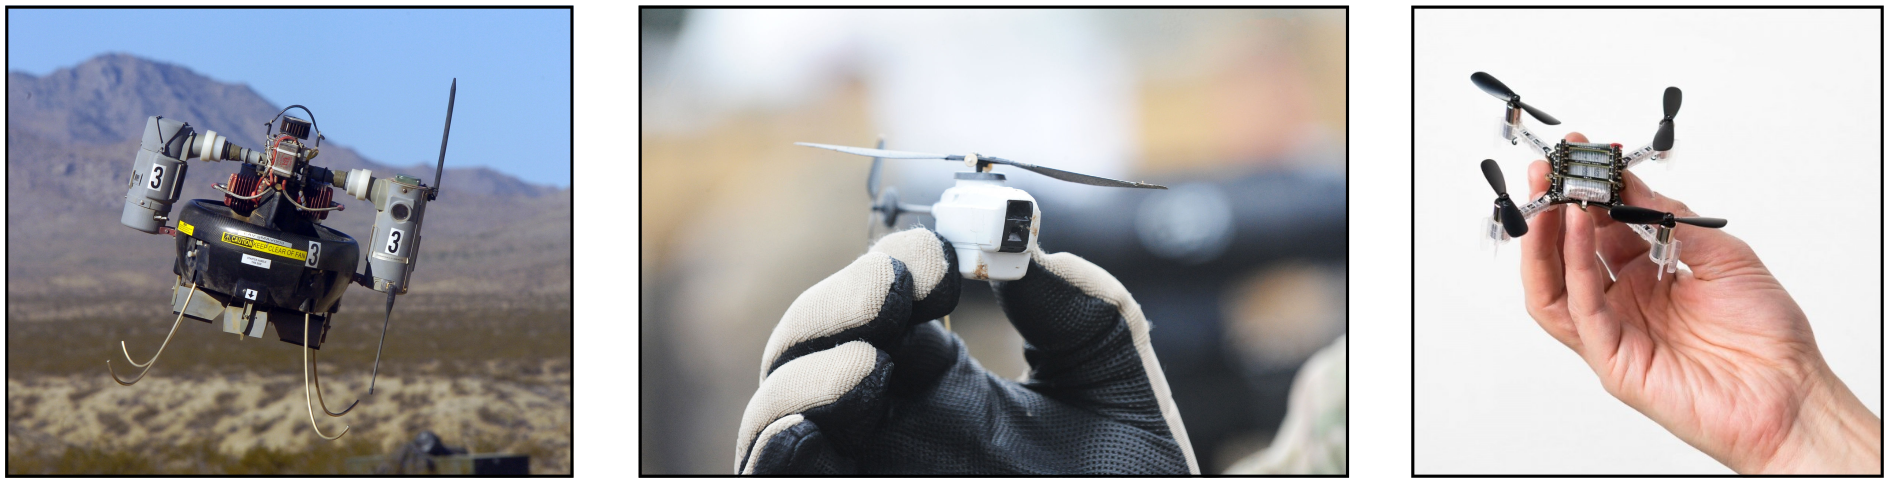
\includegraphics{Fig/intro.png}
    \caption{Micro aerial vehicles: RQ-16 T-Hawk (left), Black Hornet Nano (center), and Bitcrcaze Crazyflie 2.1 (right).}
    \label{fig:intro}
\end{figure}

At AIMotion Lab of ELKH SZTAKI there is a flying arena with five Bitcraze Crazyflie 2.1 miniature quadrotors. These drones are designed for research and education purposes, therefore they are both open hardware and open source, making it possible to implement our own algorithms on-board. Due to their low weight and relatively small mechanical power no on-board cameras can be used, therefore an external OptiTrack motion capture system provides position and orientation information for the drone, the data of which is fed back to the on-board controller via radio communication. With the highly reliable and precise localization, the Crazyflie is able to track complex trajectories with high performance using a suitable flight controller.

Backflipping with a quadcopter is an interesting control problem both from theoretical and application point of view. Flying vehicles are often subject to significant disturbances (e.g. strong wind or collision) which results in being upside-down. The recovery from that state is very complex, but a quadcopter that can perform a backflip has a higher chance to regain stability and follow its mission. From theoretical point of view, the problem is interesting not only because it emphasizes the nonlinearity of the dynamical model, but also requires special considerations regarding the attitude representation and control. 

In the literature, there are several different approaches to perform the flip maneuver. In \cite{energy-quaternion}, energy-based control is applied to overcome the uncontrollability of the quadcopter at singular configurations to follow a circular or clothoidal reference trajectory. Machine learning approaches are utilized in many cases, for example to imitate the maneuver performed by an expert drone pilot with apprenticeship learning \cite{abbeel2010}, or design time-optimal trajectories with deep reinforcement learning \cite{drone-racing-deep-rl} and learn acrobatic maneuvers \cite{deep_acrobatics, quadrotor-control-rl}. 

A simple learning strategy for adaptive open-loop control is proposed in \cite{LSICRA2010}, based on the optimization of a parametric motion primitive sequence. As backflipping pushes the actuators of the quadcopter to their physical limits, the application of near-maximal and minimal control inputs are required. This approach builds on the theory of bang-bang control and first-principles motion primitive design to perform and optimize the flip maneuver. 

Geometric control is a nonlinear approach for attitude feedback control of rigid bodies in 3D space. In \cite{lelemc2010}, it is theoretically proven that geometric control is able to stabilize the orientation of a quadcopter in the whole operating domain based on differential geometric considerations and Lyapunov stability. A control law is proposed, on which other researchers build and extend for real-time trajectory generation and aggressive, agile maneuvering \cite{turpinkumar2011, mellinger2011} .

% have a wide range of industrial applications. Most common are search and rescue missions in disaster areas, or agricultural monitoring. It is also a popular topic in the field of systems and control engineering, because of the simplicity of a baseline dynamical model and mechanical design. However, the precise execution of aggressive, fast maneuvers requires advanced modelling and control techniques, which include the use of nonlinear or learning algorithms.


In this work, firstly the theoretical background of quadrotor dynamics and control is demonstrated. In Sections 3-4, two control approaches are proposed to perform a flip maneuver:  open-loop control based on motion primitive optimization, and geometric tracking control for an optimized reference trajectory. In Section 5, the simulation framework, implementation and results are discussed for the dynamical model of the Crazyflie 2.1 quadcopter. The experimental setup, implementation on the real robot, and  measurement results are demonstrated in Section 6, with a comparison of the two control approaches. Finally, the conclusion and future work are summarized in Section 7.

\section{Mathematical model of a quadcopter}\label{sec:model}
In this section, the mathematical model of a quadcopter is presented, mainly based on \cite{quad_model}. Firstly, the coordinate frames are characterized to describe the position and orientation of the drone. The dynamic equations are then written in these frames for translational and rotational motion using multiple attitude representations. Finally, the input equations are described mapping between the control inputs and propeller angular velocities.

\subsection{Coordinate frames}\label{sec:frames}
There are two main approaches to characterize the quadcopter coordinate frames, namely '$\times$' and '+' configurations. Due to the practicality of on-board camera placement the earlier is more common, therefore we use '$\times$' configuration in this work. With choosing one of the two configurations, three main frames are used: the inertial frame $\mathcal{F}^i$ interpreted as NED (north-east-down) coordinates, the vehicle frame $\mathcal{F}^v$, and the body frame $\mathcal{F}^b$, which is fixed to the vehicle. The three frames are displayed in Figure~\ref{fig:frames}, with the body frame both in 'X' and '+' configuration. The transformation from $\mathcal{F}^i$ to $\mathcal{F}^v$ is a translation, and from $\mathcal{F}^v$ to $\mathcal{F}^b$ a rotation. In the figure, the rotation is described by the roll, pitch, and yaw (RPY) Euler angles, denoted by $\phi$, $\theta$, and $\psi$, respectively. However, we will also present other techniques to characterize this rotation in Section \ref{sec:rotation}.

\begin{figure}[b]
\centering 
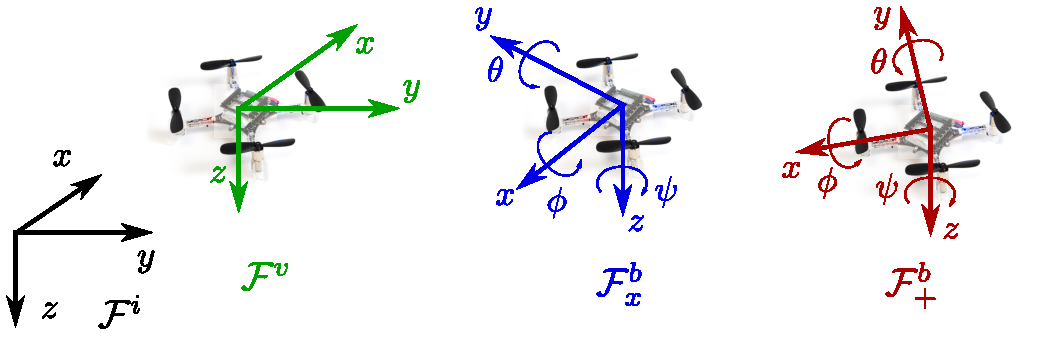
\includegraphics[width=.75\textwidth]{Fig/xconf.pdf}
\caption[Inertial, vehicle, and body frames]{Inertial, vehicle, and body frames describing the geometric relations of the vehicle and the environment. The body frame is depicted both in '$\times$' and '+' configurations.}\label{fig:frames}
\end{figure}

The matrix representation of the transformation between the vehicle and body frames can be derived from the RPY angle representation as follows:
\begin{equation}\label{eq:rot}
\begin{split}
R_v^b& = Rot(x,\phi)Rot(z,\theta)Rot(z,\psi) = \\
&=\left[\begin{array}{ccc}1 & 0 & 0 \\ 0 & C_ \phi &  S_ \phi \\ 0 & - S_ \phi & C_ \phi\end{array}\right]\left[\begin{array}{ccc} C_ \theta & 0 &  -S_ \theta \\ 0 & 1 & 0 \\  S_ \theta & 0 &  C_ \theta\end{array}\right]\left[\begin{array}{ccc} C_ \psi & S_ \psi & 0 \\ - S_ \psi &  C_ \psi & 0 \\ 0 & 0 & 1\end{array}\right]=\\
&=\left[\begin{array}{ccc} C_\psi C_\theta &  C_\theta S_\psi & -S_\theta \\
C_\psi S_\phi S_\theta - C_\phi S_\psi & C_\phi C_\psi + S_\phi S_\theta S_\psi & S_\phi C_\theta \\
S_\phi S_\psi + C_\phi C_\psi S_\theta & C_\phi S_\theta S_\psi - C_\psi S_\phi & C_\phi C_\theta
\end{array}\right],     %\left[\begin{array}{ccc} C_\psi C_\theta &  C_\theta S_\psi+ C_\psi S_\phi S_\theta &  S_\phi S_\psi- C_\phi C_\psi S_\theta \\ -C_\theta S_\psi &  C_ \phi C_ \psi - S_\phi S_\psi S_\theta & C_\psi S_\phi + C_\phi S_\psi S_\theta \\ S_\theta &  -C_\theta S_ \phi &  C_ \phi C_\theta\end{array}\right],
\end{split}
\end{equation}
where $C_\cdot = \cos(\cdot)$, $S_\cdot = \sin(\cdot)$, and $R_v^b$ is called the rotation matrix. The coloumn vectors of the rotation matrix formulate an orthonormal basis of the 3D space, therefore
\begin{equation}
R_b^v = \left(R_v^b\right)^{-1} = \left(R_v^b\right)^\top.
\end{equation}

\subsection{Translational dynamics}\label{sec:trans}

The vehicle can be modelled as a rigid body with mass and inertia in the 3D space, on which gravity field acts. The active movement of the drone is generated by  four electric motors and the propellers on them. They produce a collective thrust applied in the center of mass of the vehicle, and three moments around the three coordinate axes.

The translational dynamics of the quadcopter are characterized by Newton's equations of motion, generally expressed as
\begin{equation}\label{eq:newton}
f= m\frac{\mathrm{d} V}{\mathrm{d} t_i},
\end{equation}
where $f$ is the vector of forces acting on the mass $m$, and $V$ is the velocity of the mass. The notation $t_i$ expresses that the derivative is calculated with respect to the inertial frame.

In our model, there are two forces acting on the vehicle: the collective thrust generated by the motors, and the force of the gravitational field. The collective thrust always points in the negative $z$ direction of the body frame, and gravity always points in the positive $z$ direction of the inertial frame. The force vector in \eqref{eq:newton} results from these terms, as
\begin{equation}\label{eq:newtoneq}
f = R_b^v\begin{bmatrix} 0\\0\\-F \end{bmatrix} + \begin{bmatrix} 0\\0\\mg \end{bmatrix},
\end{equation}
where $F$ is the collective thrust of the propellers, and $g$ is the gravitational acceleration.

\subsection{Rotational dynamics} \label{sec:rotation}

There are multiple ways to describe the rotational motion of a rigid body in 3D space, out of which three approaches will be presented in this work. The most common and simple way is to use local coordinates, i.e. describe the attitude with three axes, and three rotation angles around them. An example is the RPY angle representation mentioned in Section \ref{sec:frames}, where the three axes are the body $z, y, x$ axes, and the three angles are the yaw ($\psi$), pitch ($\theta$) and roll ($\phi$), respectively. Although this approach is intuitive and commonly used, it has two major drawbacks. The first is that it is only valid in a certain region of the attitude, for example $-\pi/2 \leq \phi \leq \pi/2,\; -\pi/2 \leq \theta \leq \pi/2,\; 0 \leq \psi \leq 2\pi$. The second is the so called \textit{gimbal lock}, meaning that a degree of freedom is lost if two axes become parallel out of the three. In case of the flip maneuver, when the pitch is 90 degrees, the yaw axis is parallel to the roll axis, and the compensation for the yaw changes is not possible. Due to these drawbacks, in quadcopter navigation we use RPY (or Euler) angles only for slower maneuvering and trajectory tracking, but in case of an aggressive maneuver, there are more efficient approaches.

Another possible representation of rigid body rotations is using orientation quaternions. In this case, there is no need to deal with the gimbal lock, and a continuous trajectory can be described by a continuous function of the quaternion elements. However, unit quaternions are ambiguous, as they double-cover the rotation group $SO(3)$, meaning that quaternions $q$ and $-q$ represent the same rotation, which causes difficulties in control design. Therefore we will only use this representation for trajectory design.

The third representation of orientation we describe is the rotation matrix. Any rigid body rotation can be characterized by a $3\times 3$ orthogonal matrix with determinant 1. These matrices form the configuration space of the orientation of a non-symmetrical object in 3D space, named the special orthogonal group, $SO(3)$. Advantages of this approach are that the product of two rotations is the composition of the rotations, therefore the orientation can be given as the rotation from an initial frame to a current body frame, and it avoids singularities and complexities arising when using local coordinates. The disadvantages of using orientation matrices are that the use of 9 variables (elements of a $3\times 3$ matrix) is computationally less efficient than 3 angles or 4 quaternion elements, and they are less illustrative.

In this section, the rotational dynamics of the quadrotor will be derived using all three mentioned representations, in order to be able to use them for trajectory planning and control design. The translational dynamics from Section \ref{sec:trans} and the rotational dynamics with one of the three attitude representations together characterize the dynamic model of the quadcopter.





\subsubsection{Euler angles}
The orientation is described with the vector of roll, pitch and yaw angles, $[\phi,\theta,\psi]^\top$. However, since the three rotations are in different frames, the vector of derivatives of the three angles is not equal to the derivative of the vector of the angles. We denote the former $[\dot\phi,\dot\theta,\dot\psi]^\top$, and the latter $[p,q,r]^\top$. The relation of these vectors is described by a matrix transformation, as
\begin{align}
\begin{bmatrix} p\\q\\ r \end{bmatrix} &= \begin{bmatrix}
1 & 0 & -\sin\theta \\ 
0 & \cos\phi & \cos\theta\sin\phi \\ 
0 & -\sin\phi & \cos\theta\cos\phi
\end{bmatrix}\begin{bmatrix}
\dot\phi \\ \dot\theta \\ \dot\psi
\end{bmatrix} = W \begin{bmatrix}
\dot\phi \\ \dot\theta \\ \dot\psi
\end{bmatrix},\\
\begin{bmatrix}
\dot\phi \\ \dot\theta \\ \dot\psi
\end{bmatrix}&= W^{-1}\begin{bmatrix} p\\q\\ r \end{bmatrix} = \begin{bmatrix}
1 & \sin\phi\tan\theta & \cos\phi\tan\theta \\
0 & \cos\phi & -\sin\phi \\
0 & \frac{\sin\phi}{\cos\theta} & \frac{\cos\phi}{\cos\theta}
\end{bmatrix}\begin{bmatrix} p\\q\\ r \end{bmatrix}.\label{eq:angvel}
\end{align}

The rotational dynamics can be described by Euler's equations, as
\begin{equation}\label{eq:newton2}
\tau = \frac{\mathrm{d}J\omega}{\mathrm{d}t_i},
\end{equation}
where $\tau$ is the torque acting on the body, $J$ is the inertia, and $\omega$ is the angular velocity. The rotation is easier to express in the body frame, as the $J^b$ inertia is constant, and the angular velocity is $\omega^b = [p,q,r]^\top$. However, as the derivatives in \eqref{eq:newton2} are calculated with respect to the inertial frame, the formulae of derivation in a moving frame have to be applied, resulting in
\begin{align}
\frac{\mathrm{d}J^b\omega^b}{\mathrm{d}t_i}&= \frac{\mathrm{d}J^b\omega^b}{\mathrm{d}t_b} + \left(\omega^b\times J^b \omega^b\right)=\underbrace{\frac{\mathrm{d}J^b}{\mathrm{d}t_i}\omega^b}_{=0} + J^b \frac{\mathrm{d}\omega^b}{\mathrm{d}t_i} + \left(\omega^b\times J^b \omega^b\right) = \tau,\\
    &\Downarrow \nonumber\\
\begin{bmatrix}
\dot{p} \\ \dot{q} \\ \dot{r} 
\end{bmatrix} &= \left(J^b\right)^{-1}\left(\tau - \omega^b\times J^b \omega^b\right) .\label{eq:rot_dyn}
\end{align}

Quadcopters are almost perfectly symmetric, therefore the off-diagonal terms of the inertia matrix are usually neglected. Thus the equation for the rotational acceleration results in
\begin{equation}\label{eq:rotvel}
\begin{bmatrix}
\dot{p} \\ \dot{q} \\ \dot{r} 
\end{bmatrix} = \begin{bmatrix}
\frac{J_y-J_z}{J_x}\cdot q\cdot r + \frac{\tau_x}{J_x} \\ \frac{J_z-J_z}{J_x}\cdot p\cdot r + \frac{\tau_y}{J_y} \\ \frac{J_x-J_y}{J_z}\cdot p\cdot q  + \frac{\tau_z}{J_z}  
\end{bmatrix}.
\end{equation}

The drone as a rigid body in 3D space has 12 states: the position, velocity, rotation and rotational velocity. The equations for the velocity are from \eqref{eq:rot} and \eqref{eq:newtoneq}, for the rotation from \eqref{eq:angvel}, and for the rotational velocity from \eqref{eq:rotvel}. Gathering these to a matrix form, the following state space representation is formulated:
\begin{equation}\label{eq:ss}
\begin{bmatrix}
\dot{x} \\ \dot{y} \\ \dot{z} \\ \dot{V_x} \\ \dot{V_y} \\ \dot{V_z} \\ \dot{\phi} \\ \dot{\theta} \\ \dot{\psi} \\ \dot{p} \\ \dot{q} \\ \dot{r}
\end{bmatrix} = \begin{bmatrix}
V_x \\ V_y \\ V_z \\ -(\sin \phi \cdot \sin \psi+\cos \phi \cdot \cos \psi \cdot \sin \theta) \frac{F}{m} \\
-(\cos \phi \cdot \sin \psi \cdot \sin \theta-\cos \psi \cdot \sin \phi) \frac{F}{m} \\
-(\cos \phi \cdot \cos \theta) \frac{F}{m}+g \\
p+\sin \phi \cdot \tan \theta \cdot q+\cos \phi \cdot \tan \theta \cdot r \\
\cos \phi \cdot q-\sin \phi \cdot r \\
\frac{\sin \phi}{\cos \theta} \cdot q+\frac{\cos \phi}{\cos \theta} \cdot r \\
\frac{J_{y}-J_{z}}{J_{x}} \cdot q \cdot r+\frac{\tau_{x}}{J_{x}} \\
\frac{J_{z}-J_{x}}{J_{y}} \cdot p \cdot r+\frac{\tau_{y}}{J_{y}} \\
\frac{J_{x}-J_{y}}{J_{z}} \cdot p \cdot q+\frac{\tau_{z}}{J_{z}}
\end{bmatrix}.
\end{equation}


\subsubsection{Quaternion based model}
%The so far described RPY representation is only valid for a certain region of the angles, i.e. $-\pi/2 \leq \phi \leq \pi/2,\; -\pi/2 \leq \theta \leq \pi/2,\; 0 \leq \psi \leq 2\pi$. It is sufficient in most cases, e.g. following a path or slower maneuvering, but in case of an aggressive maneuver, another approach would be more convenient. Using quaternions for describing rotations is a possible solution for the problem \cite{quaternion,energy-quaternion}. 
The second presented approach for rigid body attitude representation is using orientation quaternions. A quaternion is a hyper complex number of rank 4, which can be represented in multiple forms, see for example equation \eqref{eq:q1}. The quaternion elements from $q_1$ to $q_3$ are called the vector part of the quaternion, while $q_0$ is the scalar part.
\begin{align}
    q = q_0 + q_1\mathbf{i} + q_2\mathbf{j} + q_3\mathbf{k} = \begin{bmatrix}q_0 & q_1 &q_2& q_3 \end{bmatrix}^\top = \begin{bmatrix}q_0 \\ \mathbf{q} \end{bmatrix} \label{eq:q1}
\end{align}
Quaternions have a special multiplication operator, denoted by $\otimes$. If $p$ and $q$ represent rotations, $p\otimes q$ represents the combined rotation. Just as the rotation, quaternion product is not commutative. Two possible (equivalent) methods for calculating this product are the following.
\begin{align}
    p\otimes q &= \underbrace{p_0 q_0 - \mathbf{p}\cdot\mathbf{q}}_{\mathrm{scalar\; part}} +\underbrace{p_0 \mathbf{q} +q_0\mathbf{p} + \mathbf{p}\cross\mathbf{q}}_{\mathrm{vector\; part}},\\
    p\otimes q &= Q(p) q=\left[\begin{array}{cccc}
p_{0} & -p_{1} & -p_{2} & -p_{3} \\
p_{1} & p_{0} & -p_{3} & p_{2} \\
p_{2} & p_{3} & p_{0} & -p_{1} \\
p_{3} & -p_{2} & p_{1} & p_{0}
\end{array}\right]\left[\begin{array}{l}
q_{0} \\
q_{1} \\
q_{2} \\
q_{3}
\end{array}\right] = \left[\begin{array}{l}
p_{0} q_{0}-p_{1} q_{1}-p_{2} q_{2}-p_{3} q_{3} \\
p_{0} q_{1}+p_{1} q_{0}+p_{2} q_{3}-p_{3} q_{2} \\
p_{0} q_{2}-p_{1} q_{3}+p_{2} q_{0}+p_{3} q_{1} \\
p_{0} q_{3}+p_{1} q_{2}-p_{2} q_{1}+p_{3} q_{0}
\end{array}\right].
\end{align}

Rotations are defined by unit quaternion products, i.e. the definition of a norm is necessary, as
\begin{align}
    \norm{q} = \sqrt{q_0^2+q_1^2+q_2^2+q_3^2}.
\end{align}
The complex conjugate of a quaternion will also be needed, defined as
\begin{align}
    q^* = \begin{bmatrix}q_0 & -q_1 & -q_2 & -q_3 \end{bmatrix}^\top.
\end{align}
Given that the angular velocity is in the body frame, the derivative of the quaternion rotation in the dynamic equations has the form \cite{quaternion}
\begin{align}
    \dot{q} =-\frac{1}{2} \omega^b \otimes q.
\end{align}
It is worth noting that if we apply the quaternion product to a $\mathbb{R}^3$ vector and a quaternion, the scalar part of the vector is always considered zero.

The rotation in \eqref{eq:newtoneq} can be characterized by two quaternion products, namely
\begin{align}
    f = q\otimes\begin{bmatrix}0 \\ 0 \\ -F\end{bmatrix}\otimes q^* + \begin{bmatrix}0 \\ 0 \\ mg\end{bmatrix},
\end{align}
where $q$ is the rotation quaternion between the inertial and body frame.

The state space representation using \eqref{eq:ss} and the above expressions has the following form:

\begin{equation}\label{eq:quatss}
\def\arraystretch{1.5}
\begin{bmatrix}
\dot{r} \\ \dot{V} \\ \dot{q} \\ \dot{\omega}^b
\end{bmatrix} = \left[\begin{array}{c}
V \\ q\otimes\frac{1}{m}\def\arraystretch{1}\begin{bmatrix}0 \\ 0 \\ -F \end{bmatrix}\otimes q^* + \begin{bmatrix}0 \\ 0 \\ g\end{bmatrix} \\ -\frac{1}{2} \omega^b \otimes q \\\left(J^b\right)^{-1}\left(\tau - \omega^b\times J^b \omega^b\right)
\end{array} \right].
\end{equation}

\subsubsection{Quadcopter model on $SE(3)$}

Although it is possible to describe any rotation with quaternions, ambiguities arise when using them to represent the attitude. The third orientation representation method described is the quadcopter model on the special Euclidean group, $SE(3)$. The proper mathematical background of group theory and Lie-groups for rigid body orientation can be found for example in \cite{isidori1995nonlinear,Leethesis}. In this paper, only the most important principles are described with an emphasis on applications.

The\textit{ orthogonal group }$O(n)$ is the group of $n\times n$ orthogonal matrices, with the following property: 
\begin{align}
    A\in O(n) \Leftrightarrow AA^\top=I,
\end{align}
where $A$ is an $n\times n$ matrix. The column vectors of these matrices are orthogonal, and their determinant is always either 1 or $-1$. The\textit{ special orthogonal group} $SO(n)$ is the subgroup of orthogonal matrices, in which every matrix has determinant 1. These matrices can represent rotations in $n$-dimensional space, therefore they are named rotation matrices.

In order to represent both translations and rotations, $SO(n)$ needs to be extended. Consider the set of all $(n+1)\times (n+1)$ transformation matrices of the form
\begin{align}
    \left\{ \begin{pmatrix}R & v \\ 0 & 1  \end{pmatrix} \;\bigg\vert\; R \in SO(n) \mbox{ and } v \in {\mathbb{R}}^n \right\}.
\end{align}
The matrix $R$ achieves the rotation, and the vector $v$ the translation. The result is the \textit{special Euclidean group} $SE(n)$, which is homeomorphic to $ {\mathbb{R}}^n \times SO(n)$, because the rotation matrix and translation vectors may be chosen independently.

Rigid body translation and rotation is described in the 3D space, therefore the representation is in the special Euclidean group $SE(3)$, and the rotation matrix in the special orthogonal group $SO(3)$. The attitude dynamics have a simple form using rotation matrices, namely
\begin{align}
    \dot{R} & = R\hat{\omega},\label{eq:rot1}\\
    \dot{\omega} & = J^{-1}\left(\tau - \omega\times J \omega\right),\label{eq:rot2}
\end{align}
where $R$ is the rotation matrix between the vehicle and body frames, and the \textit{hat map} $\hat{\cdot}:\mathbb{R}^3\rightarrow SO(3)$ is defined by the condition that $\hat{x}y = x\times y$ for all $x,y\in \mathbb{R}^3$. From here on the indices corresponding to the body and vehicle frames from \eqref{eq:newtoneq} and \eqref{eq:rot_dyn} are omitted for clarity, the inertia and angular velocity are always defined in the body frame. %The translational dynamics are characterized by \eqref{eq:newtoneq}, the two forces acting on the body are the collective thrust and gravitational force.

%\subsection{Differential flatness}\label{sec:flat}
%The demonstrated dynamical model of the quadcopter is underactuated as it has six degrees of freedom and only four control inputs. However, in trajectory design it is often utilized that the model is \textit{differentially flat}, i.e. all state variables and control inputs can be expressed from a finite number of time derivatives of four flat outputs, namely the position $x,y,z$ and yaw angle $\psi$. This simplifies the trajectory planning: only $x_d(t), y_d(t), z_d(t), \psi_d(t)$ have to be constructed, they determine the remaining states. 

\subsection{Input equations}


The dynamic model has four inputs: the collective thrust, and the torques around the three axes of the body frame. These inputs can be calculated from the individual thrusts and angular speeds of the actuators, the equations of which will be described in this section.

The thrust generated by each motor ($T_i$) is proportional to the square of the corresponding angular velocity ($\omega_i$), resulting in the equation
\begin{equation}
T_i = k\omega_i^2,\label{eq:thrustconstant}
\end{equation}
where $k$ is the \textit{thrust constant}. 

% \subsubsection{'X' configuration}

The direction of rotor thrust, angular velocity and the numbering of propellers are displayed in Figure \ref{fig:input_eqs}. The torques around the axes $x$ and $y$ can be calculated as the product of the thrusts $T_i$, and the distance of the motors and the center of mass of the vehicle $l$, as
\begin{align}
\tau_x &= \frac{l}{\sqrt{2}}(T_3+T_4-T_1-T_2) =  \frac{l}{\sqrt{2}} k \left(\omega_3^2+\omega_4^2-\omega_1^2-\omega_2^2\right),\\
\tau_y &= \frac{l}{\sqrt{2}}(T_1+T_4-T_2-T_3) =  \frac{l}{\sqrt{2}}k \left(\omega_1^2+\omega_4^2-\omega_2^2-\omega_3^2\right).
\end{align}
The torque around axis $z$ is calculated based on the effect, that every propeller rotates the vehicle in the opposite direction, and this rotating torque is proportional to the square of the angular velocity. Therefore rotors 1 and 3 create positive torque, and the others negative, resulting in the equation
\begin{equation}\label{eq:dragconstant}
\tau_z = b\left(\omega_1^2+\omega_3^2-\omega_2^2-\omega_4^2\right),
\end{equation}
where $b$ is the \textit{drag constant}. We can write the input equations \eqref{eq:thrustconstant}--\eqref{eq:dragconstant} in a matrix form, resulting in
\begin{align}\label{eq:inputs}
\begin{bmatrix}F \\ \tau\end{bmatrix}=\begin{bmatrix}1 & 1 & 1 & 1 \\ -\frac{l}{\sqrt{2}} &  -\frac{l}{\sqrt{2}} &  \frac{l}{\sqrt{2}} &  \frac{l}{\sqrt{2}} \\  \frac{l}{\sqrt{2}} & -\frac{l}{\sqrt{2}} &  -\frac{l}{\sqrt{2}} &  \frac{l}{\sqrt{2}} \\ \frac{b}{k} & -\frac{b}{k} & \frac{b}{k} & -\frac{b}{k}\end{bmatrix}\begin{bmatrix} k \omega_{1}^{2} \\ k \omega_{2}^{2} \\ k \omega_{3}^{2} \\ k \omega_{4}^{2}\end{bmatrix}.
\end{align}

\begin{figure}
\centering 
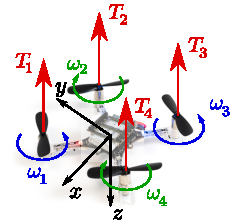
\includegraphics[width=.3\textwidth]{Fig/input_eqs.pdf}
\caption{Thrusts and angular velocities of the rotors with the body frame.}\label{fig:input_eqs}
\end{figure}

% \subsubsection{'+' configuration}
% In this case, the moments around $x$ and $y$ axes depend only on the thrust or angular velocity of two rotors, and the moment around $z$ does not differ from the previous case. The form of the equations are
% \begin{align}
% \tau_x &= l(T_4-T_2) =  l k \left(\omega_4^2-\omega_2^2\right),\\
% \tau_y &= l(T_1-T_3) = l k \left(\omega_1^2-\omega_3^2\right), \\
% \begin{bmatrix}F \\ \tau\end{bmatrix}&=\begin{bmatrix}1 & 1 & 1 & 1 \\ 0 &  -l &  0 &  l \\  l & 0 &  -l &  0 \\ \frac{b}{k} & -\frac{b}{k} & \frac{b}{k} & -\frac{b}{k}\end{bmatrix}\begin{bmatrix} k \omega_{1}^{2} \\ k \omega_{2}^{2} \\ k \omega_{3}^{2} \\ k \omega_{4}^{2}\end{bmatrix}.
% \end{align}

Since there is a constant mapping between the motor angular velocity and the vector of collective thrust and moments, we consider the $\left[F,\; \tau^\top\right]^\top$ vector the input of the system.

The identification of the input parameters $k$ and $b$ are important for accurate simulation-to-reality transfer, however, it is often difficult due to the complex aerodynamic effects, such as blade flapping and downwash. The connection of rotor angular velocity, rotor thrust and torque are often determined experimentally, resulting in more complex models than the equations described by \eqref{eq:thrustconstant} and \eqref{eq:dragconstant} \cite{Forster}.
\section{Optimization-based open-loop control}\label{sec:flip}
The flip maneuver is a 360 degree rotation around one of the horizontal axes of the quadcopter's body frame. In the literature there are several different approaches to perform the maneuver, for example based on apprenticeship learning \cite{abbeel2010}, energy-based control \cite{energy-quaternion}, or Lyapunov method \cite{lyapunov-flip}. We decided to first apply an  open-loop control method based on the optimization of a parametrized motion primitive sequence \cite{LSICRA2010}.

In this section, firstly the 2D equations of motion of the quadrotor are derived that is suitable for the applied control method. Afterwards, the parametrized primitive is described which consists of the sections of the maneuver, both beginning and ending in hover mode. Finally, the optimization problem of the primitive parameters is presented, and two different methods for the solution. 
%With the optimised parameter set, simulation results will be demonstrated. Finally, the implementation of the flip controller on the Crazyflie quadrotor, and experimental results will be discussed.

\subsection{2D Quadrotor model}

In this section, a two dimensional dynamic model of the quadcopter is used as the desired trajectory of the flip motion is within the $x-z$ plane of the body frame. The model consists of the thrust and moment of the four rotors, and the gravitational field. The rest of the dynamics is assumed to be stabilized separately so it is now ignored. Unlike the maneuver described in \cite{LSICRA2010}, we use $\times$ configuration as two rotors can produce a larger torque for the flip than one. From the Newtonian equations of motion using the direction conventions displayed in Figure \ref{fig:flipframe} and Euler angle representation:
\begin{align}
m\ddot{x}&=-(T_1 + T_2 + T_3 + T_4)\sin\theta,\\
m\ddot{z}&=-(T_1 + T_2 +T_3 + T_4) \cos\theta+mg,\\
J_{yy}\ddot{\theta} &= l(T_1+T_4-T_2-T_3),\label{eq:opinp1}
\end{align}

\begin{figure}[b]
\centering
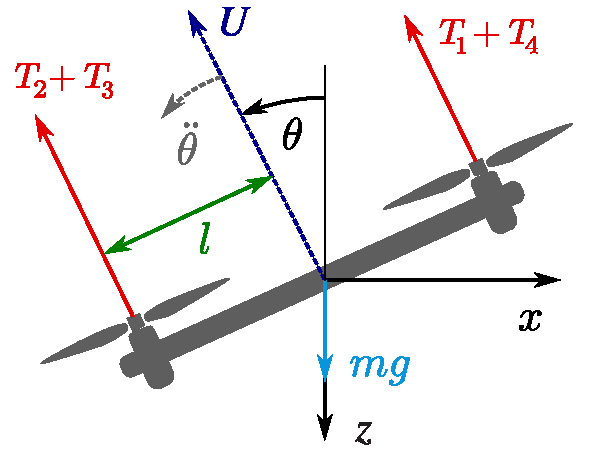
\includegraphics[width=.35\textwidth]{Fig/flip_frame_2.pdf}
\caption{The vehicle frame, the orientation and forces acting on the quadcopter in two dimensions.}\label{fig:flipframe}
\end{figure}

where $\theta$ is the pitch angle, $g$ is the gravitational acceleration, $m$ is the mass of the drone, $l$ is the distance of a propeller from the center of mass of the vehicle, $J_{yy}$ is the moment of inertia about the axis of the flip (out-of-plane principal axis), and $T_i,$ $i=1,2,3,4$ are the thrusts of each rotor. The collective acceleration $U$ is the sum of all rotor thrusts divided by the mass of the drone,
\begin{equation}
U = \frac{T_1 + T_2 + T_3 + T_4}{m}.\label{eq:opinp2}
\end{equation}
As the small DC motors of the Crazyflie 2.1 have very small time constants the actuator dynamics are omitted.% The physical parameters of the model are contained in Table x, mostly determined from \cite{Forster}.


\subsection{Parametrized primitive of the maneuver}\label{sec:sections}
The goal of the maneuver is to perform a flip, therefore the states at the start $t_0$ and end $t_f$ should be the same, except for the pitch angle which is shifted by $2\pi$. From these considerations, the initial and final state conditions for the maneuver can be formulated as follows:
\begin{subequations}
\begin{align}
x(t_0) = x(t_f) &= 0,\\
z(t_0) = z(t_f) &= 0,\\
\dot{x}(t_0) = \dot{x}(t_f) = \dot{z}(t_0) = \dot{z}(t_f) &= 0,\\
\theta(t_f) = \theta(t_0) + 2\pi &= 0.
\end{align}
\end{subequations}
We use a simple control strategy without explicit optimization for execution time. %Research has shown that for different types of dynamic systems, bang-bang control strategies provide near-optimal results, with small complexity \cite{KALMARNAGY2004,tdk2019}. 
%The actions are chosen from a restricted control envelope, denoted as a range of accelerations $[\underline{\beta},\overline{\beta}]$, in order to take into consideration modelling uncertainties and reserve some resources for the on-board stabilizing controller. This restriction can be mathematically formulated for the rotating rotor thrusts as
%\begin{align}
%T_\mathrm{min} \leq \frac{m\underline{\beta}}{4}\leq F_{i} \leq\frac{m\overline{\beta}}{4} \leq T_\mathrm{max}.
%\end{align}
The motion consists of five sections, all of which has two constant control inputs, the desired collective acceleration $U_\mathrm{des}$, and desired angular acceleration $\ddot{\theta}_\mathrm{des}$. These five steps are illustrated in Figure \ref{fig:sections}, and defined as follows.
\renewcommand{\baselinestretch}{0.85}\normalsize 
\begin{enumerate}
\item \textbf{Accelerate:} Gain elevation and kinetic energy with near-maximal collective acceleration, while rotating slowly to the negative direction.
\item \textbf{Start Rotate:} Increase angular velocity with torque, i.e. maximal differential thrust.
\item \textbf{Coast:} With low and uniform thrusts hold the angular velocity, wait for the drone to rotate.
\item \textbf{Stop Rotate:} Use maximal differential thrust to decrease angular velocity and stop the rotation.
\item \textbf{Recover:} Prevent the drone from falling to the ground by applying near-maximal collective thrust, and try to get back to hover mode.
\end{enumerate}
\renewcommand{\baselinestretch}{1.15}\normalsize

\begin{figure}
\centering
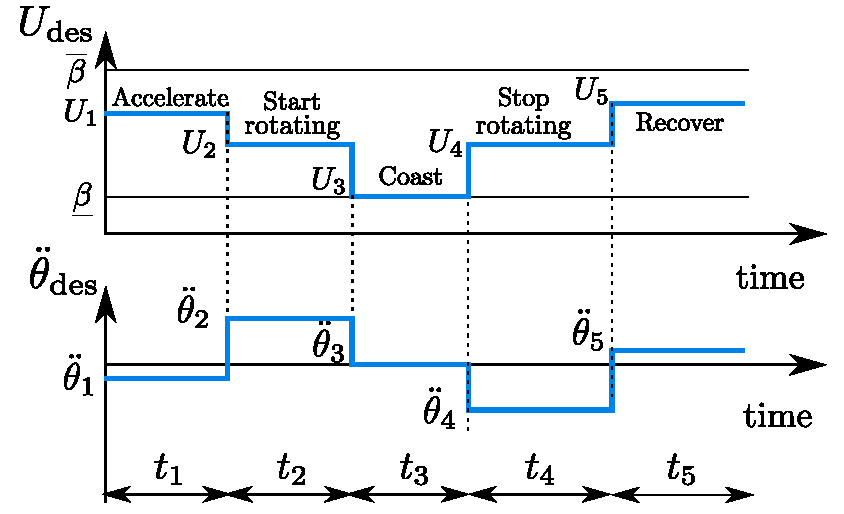
\includegraphics[scale=.7]{Fig/sections2.pdf}
\caption{Parametrized flip primitive with the five sections.}\label{fig:sections}
\end{figure}

Each of the five sections has three parameters, the collective acceleration $U_i$, duration $t_i$, and angular acceleration $\ddot{\theta}_i$, resulting in 15 parameters altogether. However, we reduce the number of parameters using bang-bang type control on a restricted control envelope. The bang-bang approach means that the control actions $U_i$ and $\ddot\theta_i$ are either zero or near-maximal at all sections. Following the equations detailed in \cite{LSICRA2010}, 10 parameters out of 15 can be expressed using the properties of bang-bang control. The remaining 5 independent parameters are optimized to perform the desired backflip motion. The vector of these parameters is characterized as follows:
\begin{align}
p=\begin{bmatrix}\label{eq:openparams}
U_1 & t_1 & t_3 & U_5& t_5
\end{bmatrix} ^\top.
\end{align} 
From the elements of $p$, the control input vector can be calculated as
 \begin{align}\label{eq:openinp}
    \begin{bmatrix}
        F_i \\ \tau_i
    \end{bmatrix}=\begin{bmatrix}
        mU_i \\ 0 \\ J_{yy}\ddot{\theta}_i \\ 0
    \end{bmatrix}\quad i\in\{1,2,3,4,5\},
\end{align}   
where $m$ is the mass of the quadcopter, and the index $i$ is obtained from the current time and the duration of the sections.

The five parameters are tuned in order to minimize the norm of the final state error $e\in\mathbb{R}^5$. The optimization problem is thus characterized as follows:
\begin{subequations}\label{eq:optim}
\begin{align}
e &= \begin{bmatrix}
x(t_f) & z(t_f) & \dot{x}(t_f) & \dot{z}(t_f)& \theta(t_f)
\end{bmatrix}^\top,\\
p^* &= \argmin_p \left(e^\top e\right).
\end{align} 
\end{subequations}

\subsection{Parameter optimization via numerical simulations}

In the original paper \cite{LSICRA2010}, the numerical optimization of the five parameters in \eqref{eq:openparams} is based on iterative learning, using the approximate Jacobian matrix of the final state error w.r.t the parameter vector. However, the numerical gradient approximation has vast computational cost, because the whole maneuver needs to be simulated in every approximation step. 

Hence we have chosen Bayesian optimization which does require derivatives and is suitable for global optimization of cost functions that are expensive to evaluate \cite{frazier2018tutorial, bayesopt2, brochu2010tutorial}. The general optimization problem is formulated as
\begin{equation}
    \max_{x\in A} f(x),
\end{equation}
where $x\in \mathbb{R}^d$ is the input (in our case the parameters $p$), $A$ is the feasible set typically given as a hyper-rectangle $\{x:a_i\leq x_i \leq b_i\}$, and $f$ is the objective function. Note that \eqref{eq:optim} is a minimization problem, thus we will use the negative objective function in Bayesian optimization.

The main concept of Bayesian optimization is to evaluate the unknown objective function at limited number of points, fit a surrogate parametric model on the data and optimize the surrogate model instead of the original objective function. The optimization is performed iteratively, where in each step a new test point is assigned, the objective function is evaluated at these points and the surrogate model is updated. The optimization stops if the maximum is reached with high confidence or the iteration reaches a certain number of evaluations. 

There are multiple approaches to define the surrogate parametric model, the most common of which is using \textit{Gaussian processes} (GPs) \cite{GPMPC2019}. GP provides a flexible, nonlinear structure representing a single layer neural network, depends on relatively few parameters and its training is fast and efficient. Moreover, the covariance of GP gives a measure of the uncertainty of the approximation which is then used to systematically select the next test point of the optimizer, and thus help the balance between exploration and exploitation.

By definition, a Gaussian process $\mathcal{GP}: \mathbb{R}^{d} \rightarrow \mathbb{R}$ is a mapping that assigns to every point $x \in \mathbb{R}^{d}$ a random variable $\mathcal{G} \mathcal{P}(x) \in \mathbb{R}$ such that for any finite set $x^{(1)} \ldots x^{(n)}$ the joint probability distribution of $\mathcal{G} \mathcal{P}\left(x^{(1)}\right), \ldots, \mathcal{G} \mathcal{P}\left(x^{(n)}\right)$ is Gaussian with mean $m$ and covariance $K$, expressed as
\begin{subequations}
\begin{align}
m &=\left[m\left(x^{(1)}\right), \ldots m\left(x^{(n)}\right)\right]^{\top} \\
[K]_{i j} &=\kappa\left(x_{i}, x_{j}\right),
\end{align}
\end{subequations}
where $[\cdot]_{i j}$ denotes the $(i, j)$-th entry of a matrix and $\kappa$ is a suitable kernel function. Both the mean and kernel depend on the \textit{hyperparameters} denoted by $\theta$, which are tuned during the optimization process. The goal is to learn the objective function $f:\mathbb{R}^d \rightarrow \mathbb{R}$ using a training set generated from the function evaluations $(x, f(x))$. An intuitive interpretation of the training is to find the GP that is most probable to have generated the training set, assuming that $f$ is a sample of the GP. 

The optimization starts with model selection, i.e. choosing a suitable mean and kernel function. By subtracting the mean of the data from all elements, constant zero mean is a common choice. The kernel is the core of the GP, it characterizes the function class in which we search the objective function. For smooth functions with approximately constant characteristic length the Squared Exponential kernel is a common and good choice, but there are also more complex kernel functions, e.g. the Matérn class.

In Bayesian statistics, we suppose that every unknown variable is drawn from some \textit{prior probability distribution}. In GP regression, the prior is a multivariate normal distribution, generated by evaluating the mean and covariance function with an initial set of hyperparameters at $k$ points, formulated as
\begin{equation}\label{eq:prior}
    f(X) \sim \mathcal{N}(m_0(X),\kappa_0(X,X)),
\end{equation}
where $\mathcal{N}$ denotes the normal distribution and $X=[x^{(1)}\dots x^{(k)}]$.

Now suppose that we evaluated $f$ at $n$ points giving $X=[x^{(1)}\dots x^{(n)}]$, $\overline y =f(X) = [\overline y^{(1)}\dots \overline y^{(n)}]$, and we would like to predict the value of the objective function at a new test point $x_*$. To do so, we take the $n+1$ dimensional joint distribution $$p([y^{(1)},\dots,y^{(n)},y ] \mid [X,x_*],\theta),$$ and calculate the one dimensional conditional distribution 
\begin{equation}\label{eq:posterior}
    p(y\mid x_*,y^{(1)}=\overline y^{(1)}, \dots ,y^{(n)}=\overline y^{(n)},X,\theta ),
\end{equation}
 which is called the \textit{posterior probability distribution}. The mean of \eqref{eq:posterior} is the approximation for $f(x_*)$, and the variance gives a measure of the uncertainty of the regression. The evaluation of a GP requires only elementary matrix operations, therefore it is computationally efficient. 

So far we have not discussed the hyperparameter tuning, which is an important element of the regression. To choose the hyperparameters, the most common method is \textit{maximum likelihood estimate} (MLE). The likelihood is the probability of the observations $\overline{y}$ given the hyperparameters $\theta$, which is a multivariate normal distribution. In maximum likelihood estimation, we choose the hyperparameters such that they maximize this likelihood, formulated as follows:
\begin{equation}
    \theta^* = \argmax_\theta p(\overline{y}\mid \theta).  
\end{equation}
There are also more complex hyperparameter tuning methods, for example maximum a posteriori (MAP) estimate or the fully Bayesian approach \cite{RW2006}. Here we only detailed MLE to provide a basic understanding about the hyperparameter choosing.

%Next step of the training is hyperparameter tuning, most commonly obtained by maximizing the \textit{marginal likelihood} of the training samples with respect to $\theta$. For proper scaling, often the logarithm of the likelihood is maximized, characterized by
%\begin{align}
%\log p(\overline{y} \mid {X}, {\theta}) &=\log \int_{-\infty}^{\infty} p(\overline{y} \mid f, {X}, {\theta}) p(f \mid {\theta}) \mathrm{d} f,
%\\ &=\underbrace{-\frac{1}{2} {y}^{\top}\left({K}+\sigma_{\varepsilon}^{2} \mathbf{I}\right)^{-1} \mathbf{y}}_{\text {data-fit term }}-\underbrace{\frac{1}{2} \log \left|\mathbf{K}+\sigma_{\varepsilon}^{2} \mathbf{I}\right|}_{\text {complexity term }}-\frac{n}{2} \log (2 \pi)
%\end{align}
%where $\mathcal{T} = {(x^{(i)},\overline y^{(i)})}_{i=1}^n$ is the training set, $X=[x^{(1)}\dots x^{(n)}]$, $\overline y = [\overline y^{(1)}\dots \overline y^{(n)}]^\top$ and $p({y} \mid {X}, {\theta})$ denotes the $n$ dimensional joint Gaussian distribution of $\mathcal{GP}(x^{(1)})\dots\mathcal{GP}(x^{(n)})$. Since the gradient of the expression is easy to evaluate, a gradient ascent algorithm can be applied to maximize the marginal likelihood.

%The evaluation of a trained GP, i.e. the approximation of $f$ at a test point $x_*\in\mathbb{R}^d$ is calculated as follows. We take the $n+1$ dimensional joint distribution $$p([y^{(1)},\dots,y^{(n)},y ] \mid [X,x_*],\theta),$$ and calculate the one dimensional conditional distribution $$p(y\mid x_*,y^{(1)}=\overline y^{(1)}, \dots ,y^{(n)}=\overline y^{(n)},X,\theta ).$$ The mean of this distribution $m_*$ is the approximation for $f(x_*)$, and the variance $\sigma_*$ gives a measure of the uncertainty of the regression. The evaluation of a GP requires only elementary matrix operations, therefore it is computationally efficient.

With a trained GP model and rules for the evaluation, we need an acquisition function to determine the next test point. The goal of the acquisition function is to balance between exploration and exploitation while trying to find the global maximum. A common acquisition function is \textit{expected improvement}, defined as follows. Suppose that we have already evaluated $f$ in $n$ points, and following the objective of the optimization the last observation is the best candidate, i.e. it has the largest value. Let $f_n^* = \max_{m\leq n}f(x_m)$ be the value at this point. 

Now we would like to choose the next test point $x_*$, after which the best evaluated value will either be $f(x_*)$ or $f_n^*$. The improvement in the value of the best evaluated point is then $f(x_*)-f_n^*$ if this difference is positive, and 0 otherwise. The improvement can be written more compactly as $[f(x_*)-f_n^*]^+$, where $a^+=\max(a,0)$. We would like to choose $x_*$ to maximize the improvement, however, we do not know $f(x_*)$ before the evaluation. What we can do is to take the expected value of the improvement given the observations and choose $x_*$ to maximize it. Hence we define the \textit{expected improvement} as the posterior distribution
\begin{equation}\label{eq:ei}
    \mathrm{EI}_n(x_*):=E\left([f(x_*)-f_n^*]^+ \mid X,y\right),
\end{equation}
where $E(\cdot)$ denotes the expected value, and $X,y$ are the $n$ evaluation points and observed values of $f$. The expected improvement in \eqref{eq:ei} can be evaluated in closed form, and hence the next test point is defined as
\begin{equation}
    x_{n+1} = \argmax\mathrm{EI}_n(x_*),
\end{equation}
the point with largest expected improvement. In the literature, there are other common acquisition functions, e.g. knowledge gradient or entropy search \cite{frazier2018tutorial}.

After describing the steps of Bayesian optimization with Gaussian processes, we summarize the method in Algorithm \ref{alg:bayes}.
\begin{algorithm}
\caption{Basic pseudo-code for Bayesian optimization \cite{frazier2018tutorial}}
\label{alg:bayes}
\begin{algorithmic}[1]
	\State Place a Gaussian process prior on $f$ using \eqref{eq:prior}
    \State Observe $f$ at $n_0$ initial points, set $n=n_0$
    \While {$n\leq N$}
    \State Update the posterior probability distribution on $f$ using \eqref{eq:posterior}
    \State Let the next test point $x_n$ be a maximizer of the acquisition function over $x$, where the acquisition function is computed using the current posterior distribution
    \State Evaluate $f$ at the new test point, $y_n = f(x_n)$
    \State Tune the hyperparameters of the GP
    \State $n=n+1$
	\EndWhile
	\State Return a solution: either the point evaluated with the largest $f(x)$, or the point with the largest posterior mean
\end{algorithmic}
\end{algorithm}


%The function evaluations are treated as data, based on which the posterior distribution is formulated over the objective function, using Bayes' theorem. The posterior distribution is then used to evaluate the acquisition function, and determine the next query point. With the growing number of data points, the posterior distribution will be more certain about which parts of the parameter space are worth exploring and which are not. The most common acquisition function is upper confidence bound (UCB). For the oncoming function evaluation, it always chooses the point from the parameter space where the upper confidence bound of the posterior distribution is the highest. This way, it provides a balance between exploration and exploitation, because if it would stuck in a local maximum, the confidence interval will become narrow, so the algorithm will start exploring the points with high uncertainty. 

%In most cases, Gaussian Processes (GPs) are used to define the prior and posterior distributions over the objective function. Research has shown that GP models are efficient nonlinear function approximators, especially for smooth functions with radial basis function (RBF) or Matérn kernel \cite{RW2006}.

With the mathematical model of the quadcopter and a suitable optimization algorithm, it is possible to simulate the maneuver with different parameter sets, optimize the motion, and implement on the vehicle. For the implementation of the open-loop flip, a stabilizing flight controller is also required to balance the quadcopter at the beginning and after the end of the maneuver. Setpoint stabilization is a common task in quadcopter control, a classical LTI feedback controller is suitable designed for the linearized dynamics around hovering, for example PID or LQR\cite{gym}. 

It is important to note that parameter uncertainties are the bottleneck of open-loop control strategies, it is essential to have an accurate simulation model which can be adapted to the real system in case the dynamic behaviour of the vehicle changes. In the next section, a nonlinear geometric control approach is proposed that is more robust to parameter uncertainties due to feedback, therefore does not require such complex and accurate modelling of the quadcopter dynamics.

%Although a simulation program is presented in \cite{LSICRA2010}, it is highly simplified, and created for an old Python version and a different quadrocopter. Hence we decided to use an OpenAI Gym environment based on PyBullet \cite{gym}, and implement the flip controller within this framework. As the package is originally developed for reinforcement learning with drones, it is suitable both for our current objective and future goals.
\section{Trajectory planning and geometric tracking control}

The second presented approach for performing a flip maneuver is optimization-based trajectory planning, and tracking the designed trajectory with geometric control. An important advantage of this approach compared to the open-loop control is generality, i.e. the proposed trajectory design method and motion control can be applied to a variety of different maneuvers, while the presented open-loop approach is designed specifically to the backflip maneuver.

Another important aspect is that using feedback control instead of an open-loop strategy aims to balance the negative effect of model uncertainties, external disturbances, and noise for the performance of the controller. However, classical feedback control algorithms (PID, LQR) fail for large roll and pitch angles, therefore a more complex, nonlinear control method is required. In the literature, such controllers include quaternion based attitude control \cite{quaternion}, adaptive incremental nonlinear dynamic inversion \cite{indi2015}, and machine learning approaches mainly based on deep reinforcement learning \cite{drone-racing-deep-rl,deep_acrobatics, quadrotor-control-rl}. 

Geometric control of a rigid body is similar to quaternion based control in the sense that it is nonlinear and covers the whole operating domain of the quadcopter state space. However, literature has shown that geometric control approaches have better performance and stability guarantees when following complex trajectories or performing aggressive maneuvers \cite{lelemc2010, turpinkumar2011, mellinger2011}. In this section, the trajectory planning with quaternion attitude representation and the geometric tracking control of the designed trajectory are presented.

\subsection{Geometric tracking control}
The nonlinear geometric tracking control used in this work is based on the ones presented in \cite{lelemc2010} and \cite{turpinkumar2011}, designed to track a 3D trajectory on $SE(3)$. To synthesize the control law \eqref{eq:newtoneq}, \eqref{eq:rot1} and \eqref{eq:rot2} are used to describe the dynamics of the quadcopter on $SE(3)$, gathered here for clarity:
\begin{subequations}
\begin{align}
    m\ddot{r}& = (-FR + mg)e_3,\label{eq:geom_tran}\\
    \tau& = J\dot\omega + \omega\times J \omega,\\
    \dot R &= R\hat{\omega},
\end{align}
\end{subequations}
where $r\in\mathbb{R}^3$ is the position of the drone in the inertial frame, $\omega\in\mathbb{R}^3$ is the angular velocity, $R\in SO(3)$ is the rotation matrix between the vehicle and body frames, $F\in\mathbb{R}$ is the collective thrust, and $e_3=[ 0, 0, 1 ]^\top$. The hat operator $\hat{\cdot}:\mathbb{R}^3\rightarrow SO(3)$ is defined by the condition that $\hat{x}y = x\times y$ for all $x,y\in \mathbb{R}^3$. Parameters are the mass of the drone $m$, the gravity $g$, and the inertia $J$.

Following the attitude control method proposed in \cite{lelemc2010}, the force and torque inputs $F$ and $\tau$ are defined as
\begin{subequations}\label{eq:geomlaw}
\begin{align}
    F&= (-K_r e_r - K_v e_v + m g e_3+m \ddot r_d) R e_3,\\
    \tau &= -K_R e_R - K_\omega r_\omega + \omega\times J \omega,\label{eq:geomtau}
\end{align}
\end{subequations}
with gain matrices $K_r, K_v, K_R, K_\omega \in \mathbb{R}^{3\times 3}$, and error terms
\begin{subequations}\label{eq:geomerrors}
\begin{align}
    e_r &= r-r_d,\\
    e_v &= \dot r - \dot r_d,\\
    e_R &= \frac{1}{2\sqrt{1+\mathrm{tr}\left( R_d^\top R \right)}}\left(R_d^\top R - R^\top R_d\right)^\vee,\\
    e_\omega &= \omega - R^\top R_d\omega_d,
\end{align}
\end{subequations}
where $r_d$, $R_d$ and $\omega_d$ are the position, orientation and angular velocity reference, $\mathrm{tr}(\cdot)$ is the trace operator, and the vee operator $(\cdot)^\vee$ is the inverse of the hat operator such that $(\cdot)^\vee:SO(3)\rightarrow \mathbb{R}^3$. Similarly to \cite{mellinger2011} we use diagonal matrix gains instead of scalars, because it works much better on the real system this way. With control gains selected carefully, the proposed attitude control approach is proved to be stable in the full space of rotation matrices (excluding the exact inversion), as derived in \cite{lelemc2010}.

The geometric controller demonstrated in this work has two operating modes: tracking of reference trajectories described by time functions of the flat outputs $x_d=[r_d^\top, \psi_d]^\top$ defined in Section \ref{sec:flat}, and tracking the reference flip trajectory described by time functions of the position and pitch angle. In case of trajectory planning for the flat outputs, the reference is designed such that $R_d=[r_1, r_2, r_3]$ and \cite{turpinkumar2011}
\begin{subequations}\label{eq:attref}
\begin{align}
    r_1 &= r_2\times r_3,\\
    r_2 &= \frac{r_3\times [\cos\psi_d, \sin\psi_d, 0]}{\norm{r_3\times [\cos\psi_d, \sin\psi_d, 0]}},\\
    r_3 &= \frac{-K_r e_r - K_v e_v + m g e_3+m \ddot r_d}{\norm{-K_r e_r - K_v e_v + m g e_3+m \ddot r_d}}.
\end{align}
\end{subequations}
Using the orientation reference in \eqref{eq:attref}, the third coloumn vector $r_3$ always points in the direction of the desired collective thrust, $r_2$ is always perpendicular to both $r_3$ and the desired heading direction given by $[\cos\psi_d, \sin\psi_d, 0]$, and $r_1$ is the desired heading direction, as it is perpendicular to both $r_2$ and $r_3$. Furthermore, the three coloumn vectors are of unit length at all time instants, ensuring the orthogonality of $R_d$ altogether.

However, during the flip maneuver we intend to specify $R_d$ from the pitch reference, therefore we do not use \eqref{eq:attref}, but design the trajectory such that the reference attitude is consistent with the reference position, as they are coupled in the dynamical model.  


\subsection{Trajectory planning for the flip maneuver}

Similarly to the open-loop control approach, the objective for trajectory planning is that the quadcopter should arrive as close to the starting point as possible, while keeping the control inputs within the allowed range during the maneuver. The attitude reference is specified in unit quaternions, because it is not possible to design a continuous trajectory for the flip in Euler angles, and rotation matrices are less illustrative. The conversion between Euler angles and unit quaternions is characterized by \cite{quaternion}

\begin{equation}\label{eq:eul2quat}
\begin{split}
    q =&\begin{bmatrix} q_0\\q_1\\q_2\\q_3 \end{bmatrix}={\begin{bmatrix}\cos(\psi /2)\\0\\0\\\sin(\psi /2)\\\end{bmatrix}}{\begin{bmatrix}\cos(\theta /2)\\0\\\sin(\theta /2)\\0\\\end{bmatrix}}{\begin{bmatrix}\cos(\phi /2)\\\sin(\phi /2)\\0\\0\\\end{bmatrix}}=\\=&{\begin{bmatrix}\cos(\phi /2)\cos(\theta /2)\cos(\psi /2)+\sin(\phi /2)\sin(\theta /2)\sin(\psi /2)\\\sin(\phi /2)\cos(\theta /2)\cos(\psi /2)-\cos(\phi /2)\sin(\theta /2)\sin(\psi /2)\\\cos(\phi /2)\sin(\theta /2)\cos(\psi /2)+\sin(\phi /2)\cos(\theta /2)\sin(\psi /2)\\\cos(\phi /2)\cos(\theta /2)\sin(\psi /2)-\sin(\phi /2)\sin(\theta /2)\cos(\psi /2)\\\end{bmatrix}}.
\end{split}
\end{equation}
The reference quaternion is denoted by $q_d = [q_{0d}, q_{1d}, q_{2d}, q_{3d}]^\top$, where $q_{0d}$ is the scalar part of the quaternion, and $q_{2d}$ corresponds to the pitch angle, as $q_{1d}=q_{3d}=0$, because both the roll and yaw angles are zero during the flip, $\phi=\psi=0$. Utilizing that $q_d$ is a unit quaternion, 
\begin{align}
    q_{2d} = &\sqrt{1-q_{0d}^2},
\end{align}
therefore it is sufficient to design a trajectory only for $q_{0d}=\cos(\theta/2)$. 

\begin{figure}
    \centering
    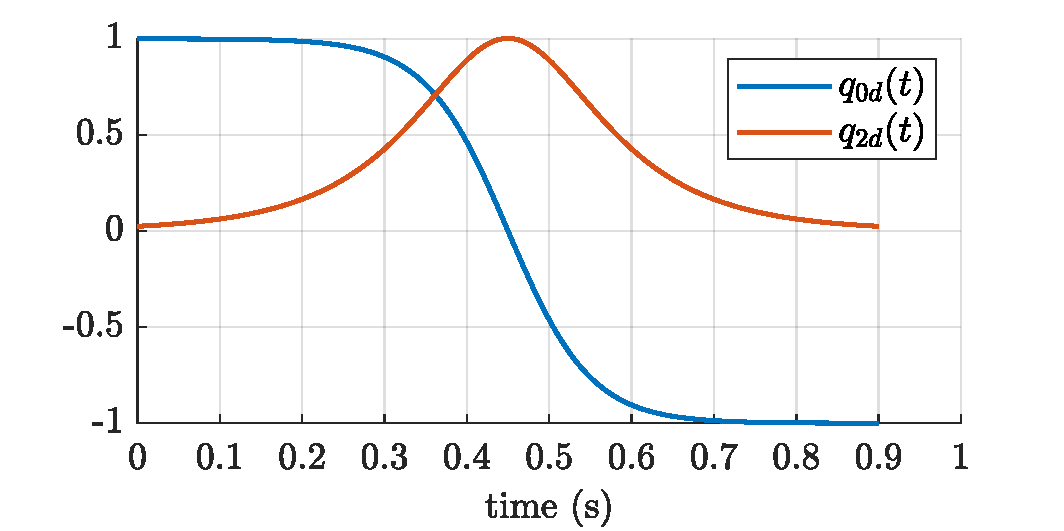
\includegraphics[width=10cm]{Fig/quat_ref.pdf}
    \caption{Attitude quaternion reference trajectory for the backflip maneuver with $\alpha=20$ 1/s, $\beta = 0.45$ s.}
    \label{fig:attref}
\end{figure}

A 360 degree turn around the pitch axis means that the scalar part of the attitude quaternion goes from 1 to -1. In the trajectory design it is important to stay within the $q_{0d}\in [-1, 1]$ range, because only unit quaternions describe rotation. We have chosen a smooth sigmoid function
\begin{equation}\label{eq:sigmoid}
    q_{0d} = \frac{2}{1+e^{-\alpha(t-\beta)}}-1
\end{equation}
to describe the scalar part of the reference attitude, where the parameters are the speed of the maneuver $\alpha$ and half of the duration of the flip $\beta$. The attitude quaternion reference trajectory is displayed in Figure \ref{fig:attref}.

The position reference need to be design considering that the rotational and translational equations of the dynamical model are coupled. The motion of the flip maneuver is within the $x-z$ plane, therefore $y_d(t) = 0$. The other two equations of \eqref{eq:geom_tran} are
\begin{subequations}\label{eq:any}
    \begin{align}
       m \ddot x & = - Fr_{13}',\\
        m \ddot{z} & = - F r_{33}' + mg,  
    \end{align}
\end{subequations}
where $r_{ij}'$ is the element of the rotation matrix $R$ in the $i$th row and $j$th coloumn. However, assuming that the attitude tracking converges fast enough to the reference, we can substitute the reference rotation matrix in \eqref{eq:any}, resulting in the translational state space representation
%\begin{subequations}
    \begin{align}\label{eq:linsys}
    \frac{\mathrm{d}}{\mathrm{d}t} \underbrace{\begin{bmatrix} x \\ \dot x \\ \tilde z \\ \dot{\tilde{z}}\end{bmatrix}}_{\mathbf{x}} = \underbrace{\begin{bmatrix} 0 & 1 & 0 & 0 \\ 0 & 0 & 0 & 0 \\ 0 & 0 & 0 & 1 \\ 0 & 0 & 0 & 0 \end{bmatrix}}_{\mathbf{A}} \begin{bmatrix} x \\ \dot x \\ \tilde z \\ \dot{\tilde{z}} \end{bmatrix} + \underbrace{\begin{bmatrix} 0 \\ r_{13}/m \\ 0 \\ r_{33}/m \end{bmatrix}}_{\mathbf{B}}  F
      % m \ddot x & = - Fr_{13},\\
      %  m \ddot{z} & = - F r_{33} + mg,  
    \end{align}
%\end{subequations}
where $r_{ij}$ are the corresponding elements of the reference rotation matrix $R_d$, converted from the reference quaternion, and $\mathbf A, \mathbf B$ are the state space matrices. As the equations are decoupled, the effect of gravity can be added to the $z$ position after a simulation, thus in the equation $\tilde{z}$ denotes the modified state. Notice that \eqref{eq:linsys} is a linear state space representation with the thrust force $F$ as the only control input. With discretizing the system, a quadratic programming problem can be formulated to a finite horizon, similarly to model predictive control.

The discrete state space model can be calculated as \cite{linearsys}
\begin{align}
    & \mathbf x_{k+1} = \mathbf A_d \mathbf x_k + \mathbf B_d u_k,\\
    & \begin{bmatrix} {\mathbf A_{d}} & {\mathbf B_{d}} \\ {\mathbf 0} & {\mathbf I} \end{bmatrix}= \mathrm{exp}\left({{\begin{bmatrix} \mathbf{A} & {\mathbf B} \\ \mathbf{0} & \mathbf{0} \end{bmatrix}}T_s}\right),
\end{align}
where $\mathbf A_d, \mathbf B_d$ are the discrete state space matrices, $\mathbf 0$ and $\mathbf I$ denote the zero and identity matrices with suitable size, $T_s$ is the sampling time and the exp$(\cdot)$ operator is the matrix exponent. The input of the model is the collective thrust of the propellers, $u_k=F_k$.

For a fixed duration of the maneuver with $N$ discrete time steps, the optimization problem is formulated as
\begin{subequations}\label{eq:quadprog}
    \begin{align}
        &\min_u \sum_{k=1}^N \left[ \left(\mathbf x_k-\mathbf x_{d,k}\right)^\top \mathbf Q_k  \left(\mathbf x_k-\mathbf x_{d,k}\right) + u_k^\top R_k u_k\right], \text{ s.t.}\\
        &\mathbf x_{k+1} = \mathbf A_d \mathbf x_k +\mathbf B_d u_k,\\
        &\{ \mathbf x_{k}\}_{k=1}^N \in \mathcal{X},\\
        &\{u_{k}\}_{k=0}^N \in \mathcal{U},
    \end{align}
\end{subequations}
where $\mathbf Q_k\in \mathbb{R}^{4\times 4}$ and $R_k \in\mathbb{R}$ are weight matrices, and $\mathcal{X}, \mathcal{U}$ are the sets of constraints for the states and the control input, respectively. In this case, we can specify linear constraints for the states, for example $x\in[x_-,x_+], z\in[z_-, z_+]$, and also linear constraint for the control input, namely
    \begin{align}
        \frac{\norm{\tau_k}}{l} \leq u_k = F_k \leq F_\mathrm{max}-\frac{\norm{\tau_k}}{l},
    \end{align}
where $\tau_k$ is the vector of the three torques around the three body axes, out of which $\tau_x=\tau_z=0$ normally during the flip, $l$ is the distance of the quadcopter center of mass and the propellers projected to the $x-z$ plane, and $F_{max}$ is the maximal collective thrust of the rotors. The torque control input $\tau_k$ is calculated from the reference attitude $R_d$ based on \eqref{eq:geomtau} assuming that the orientation and angular velocity errors are zero.

The only objective of the trajectory design is to minimize the final position error of the quadcopter and keep the position within a specified range, therefore the weight matrices are $R_k = 0, \mathbf Q_k=0$ for $k=1\dots N$, except for the weight of the final state that is
\begin{equation}
\mathbf Q_N = \begin{bmatrix} 1 & 0 & 0 & 0 \\ 0 & 0 & 0 & 0 \\ 0 & 0 & 1 & 0 \\ 0 & 0 & 0 & 0 \end{bmatrix}.
\end{equation}
As all the other weights are zero, it is only required to specify a final state position reference that is defined as
\begin{equation}
    \mathbf x_{d,N} = \begin{bmatrix} x_{d,N} \\ \dot{x}_{d,N} \\ {\tilde{z}}_{d,N} \\ \dot{\tilde{z}}_{d,N} \end{bmatrix} = \begin{bmatrix} 0 \\ 0 \\ \frac{1}{2}g(T_s N)^2 \\ 0 \end{bmatrix}.
\end{equation}

The solution of a quadratic optimization program with linear constraints is a built-in feature of most engineering programming languages, for example the \verb+quadprog+ function in Matlab. 
\section{Simulations}\label{sec:simu}
In this section, the applied simulation framework and the implemented simulations are presented for the quadrotor flip maneuver, followed by the achieved results. The simulations are based on the dynamic model of a Bitcraze Crazyflie 2.1 miniature quadcopter which we use for demonstrating the experimental results in Section \ref{sec:exp}, as well. The nonlinear equations of motion are defined in Section \ref{sec:model}, and the physical parameters of the drone are shown in Table \ref{tab:params}, obtained from \cite{Forster}.

\begin{table}[!b]
    \centering
    \setlength{\tabcolsep}{1.5pt}
    \caption{Physical parameters of the Crazyflie 2.1 quadcopter.}
    \label{tab:params}
    \begin{tabular}{|l|c|rl|}
        \hline
        \phantom{o}Mass &\phantom{o} $m$ \phantom{o}& 0.028&g \\
        \hline
        \phantom{o}Propeller-to-propeller length \phantom{o}&\phantom{o} $l$\phantom{o} & 92&mm\\
        \hline
        \multirow{3}{*}{\phantom{o}Diagonal inertia elements} & \phantom{o}$J_{xx}$\phantom{o} & $1.4\cdot 10^{-5}$&kgm$^2$\\
         \cline{2-4}
        &\phantom{o} $J_{yy}$ \phantom{o}& $1.4\cdot 10^{-5}$&kgm$^2$\\
        \cline{2-4}
        & \phantom{o}$J_{zz}$\phantom{o} & \phantom{o}$2.17\cdot 10^{-5}$&kgm$^2$\phantom{o}\\
        \hline
        \phantom{o}Thrust coefficient & $k$ & $2.88\cdot 10^{-8}$ & Ns$^2$\\
        \hline
        \phantom{o}Drag coefficient & $b$ & \phantom{o}$7.24\cdot 10^{-10}$ & Nms$^2$\phantom{o}\\
        \hline
    \end{tabular}
\end{table}

After some literature survey about drone simulators such as \cite{airsim2017} and \cite{flightmare2020}, we decided to choose an OpenAI Gym environment based on PyBullet \cite{gym}. This framework is written in Python language, contains the physical model and parameters of the Bitcraze Crazyflie 2.1, has built-in multi-agent control, and tuned PID controller for the drone. There are also some simple examples for trajectory tracking, and reinforcement learning with a swarm of drones.

All of the simulation code used in this work is available at GitHub\footnote{\url{https://github.com/antalpeter1999/TDK2021}}, the Python code is in the simulations/crazyflie-demo-simulation repository, and the Matlab code is in the trajectory-design repository. A video illustrating the simulation results is available at \url{https://youtu.be/AhqfXZ-CPqM}. In this section and the oncoming sections, we plot the measurement results with the $z$ axis pointing upwards (in contrast to the NED convention discussed in Section \ref{sec:model}), because the backflip maneuver is more illustrative this way.

\subsection{Optimized open-loop control}\label{sec:opensimu}
Based on the control approach presented in Section~\ref{sec:flip}, we implemented the open-loop flip controller which evaluates the five sections of the parametrized motion primitive. For the optimization of the parameters defined in \eqref{eq:openparams}, we utilize the Bayesian Optimization Python module \cite{bayesopt}.% The source code is available at \url{https://github.com/antalpeter1999/gym-pybullet-drones-0.5.2}.

The simulation starts with hovering for about 0.1 s, followed by executing the open-loop maneuver, and then switching back to PID control to stabilize the drone and bring back to the initial setpoint. The objective function of the optimizer uses the same simulation, and returns the norm of the final state error, as it is characterized in \eqref{eq:optim}. The optimal parameters were calculated with Bayesian optimization, using 250 random initial function evaluations and 1000 iterations. The numerical values of these are
\begin{align}\label{eq:optparam}
P^*=\begin{bmatrix}
U_1^* & t_1^* & t_3^* & U_5^*& t_5^*
\end{bmatrix} ^\top =  \begin{bmatrix}
17.5 & 0.12 & 0.16 & 17.95 & 0.075
\end{bmatrix}^\top,
\end{align}
where the unit of the collective accelerations $U_i^*$ is m/s$^2$, and the time is in seconds. It is simple to convert the collective acceleration to collective thrust, 
\begin{equation}
    F = m U,
\end{equation}
where $m$ is the mass of the quadcopter. Simulation results are displayed in Figure \ref{fig:opensimu}, using the optimal parameter vector and a set of near-optimal parameters, as well. On the left plot, the position of the quadcopter during the flip is shown, with snapshots from the simulation. The end of the optimal maneuver is around the coordinate $(x, z)=(-0.4, 0)$~m with near-zero pitch angle, thus the final state error is only significant in the $x$ position. From that point, a PID controller\cite{gym} stabilizes the drone and controls to the origin. On the right, the trajectory of the pitch angle in Euler representation, the angular velocity, and the collective thrust as a control input are shown, where the five sections defined in Section~\ref{sec:flip} can be recognised clearly. The figure illustrates that even small deviations from the optimal parameter set (<10\%) result in significantly decreasing performance.

\begin{figure}[!h]
\centering
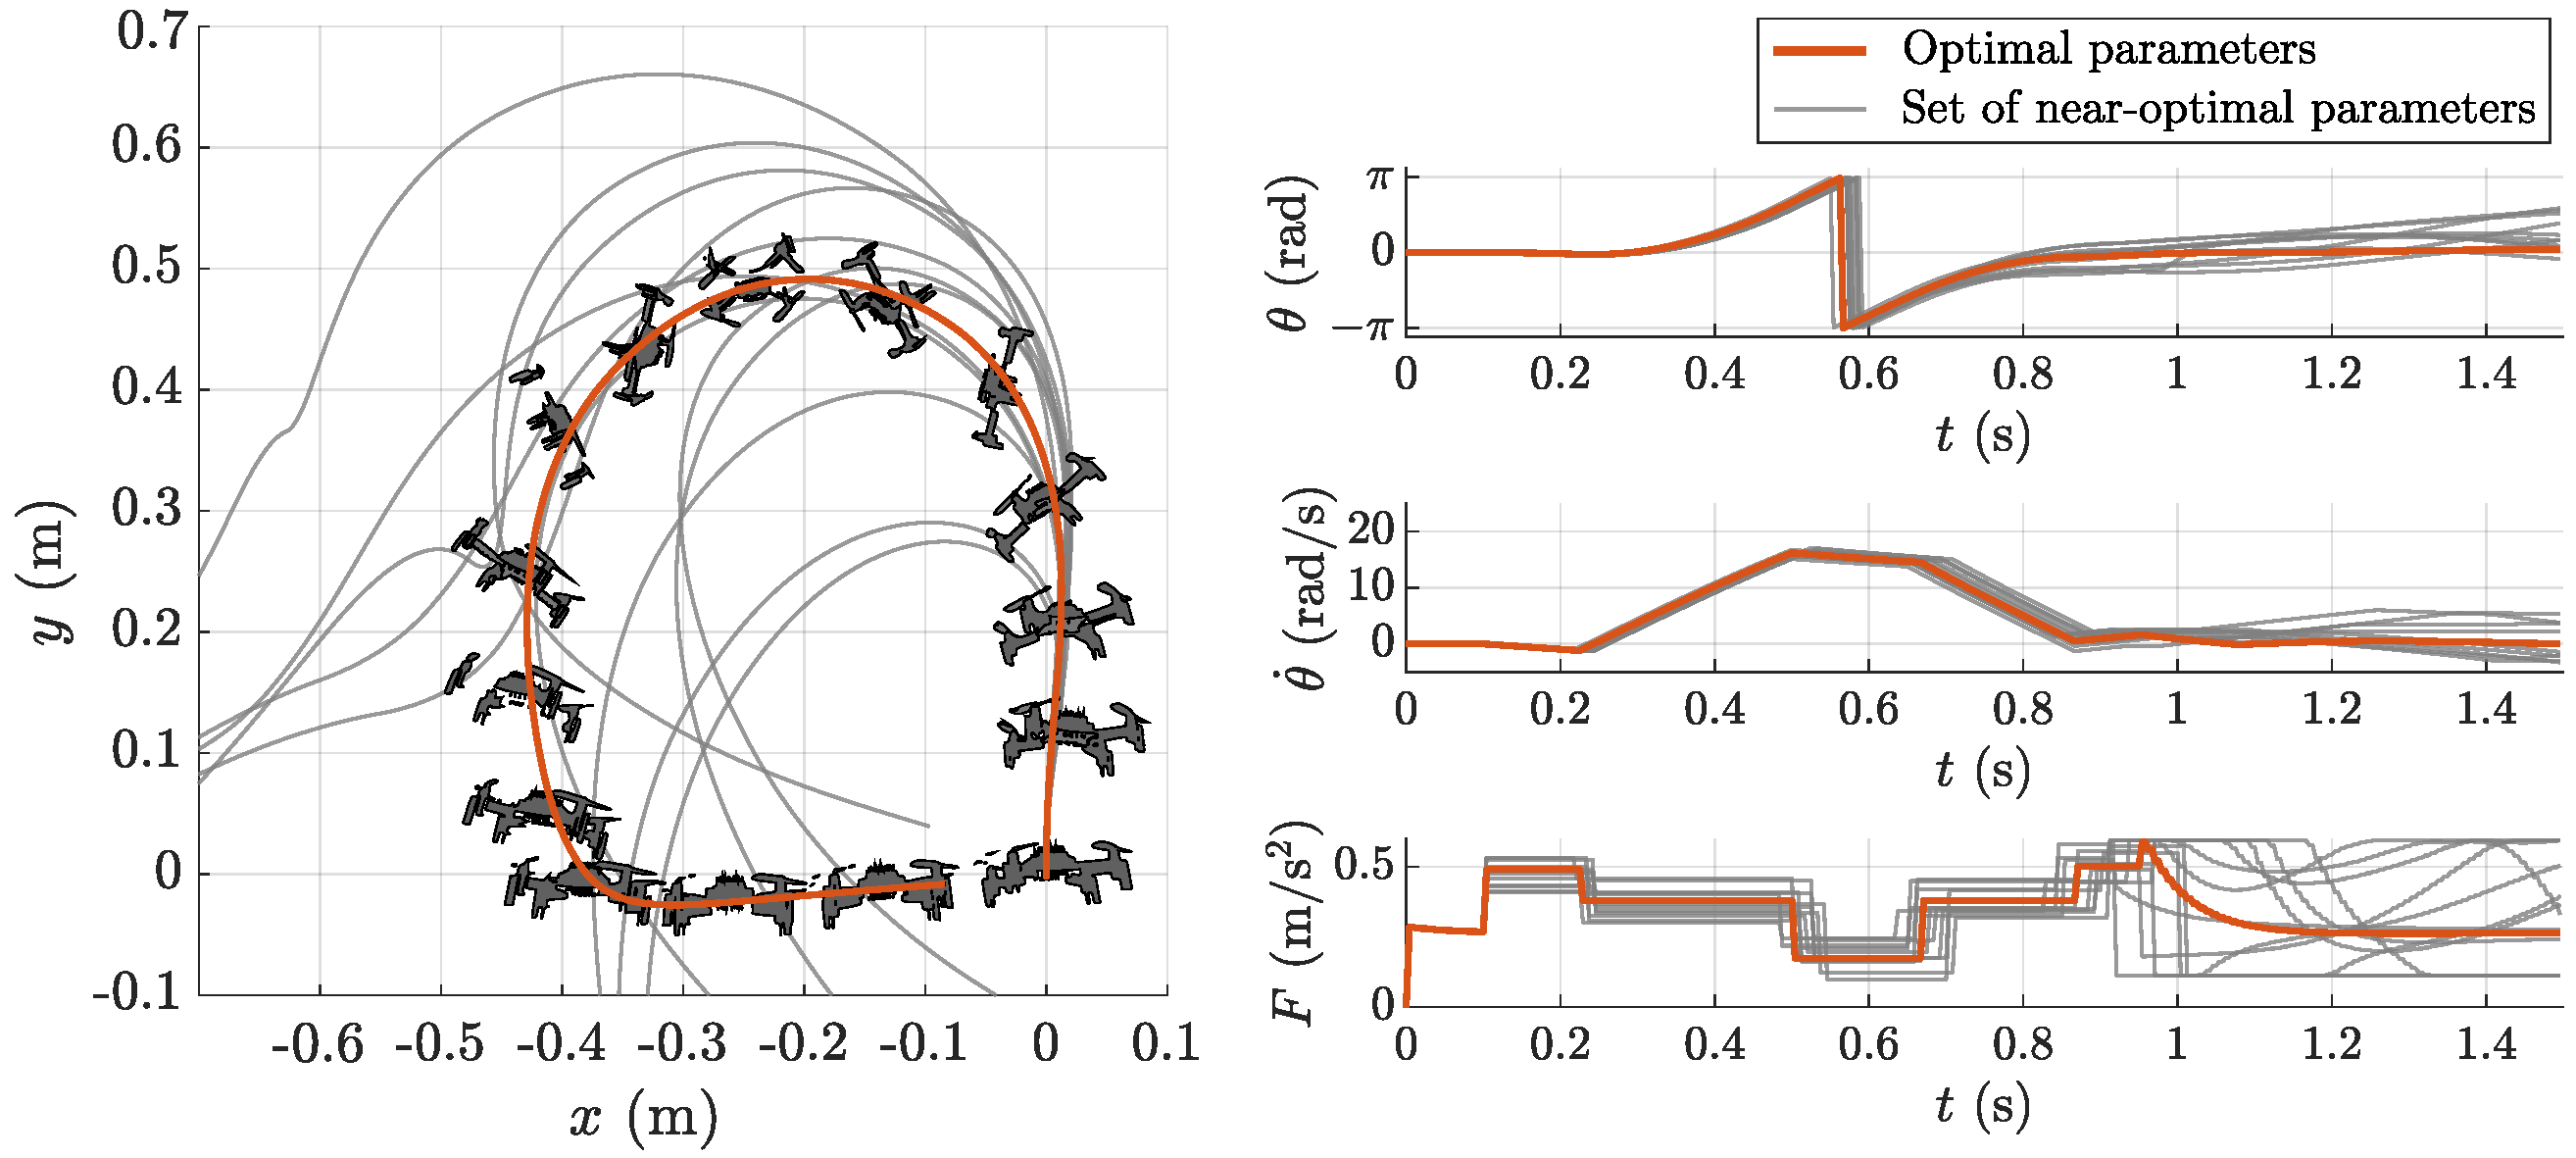
\includegraphics[width=\linewidth]{Fig/opensimu2.pdf}
\caption[Open-loop backflip simulation results]{Open-loop backflip simulation results: the position is displayed on the left, and the pitch angle $\theta$, pitch angular velocity $\dot{\theta}$, and collective thrust $F$ on the right. Orange lines represent the simulation with optimal parameters in \eqref{eq:optparam}, and grey lines represent the result of small changes in the parameter set.}\label{fig:opensimu}
\end{figure}



%\begin{figure}
%\centering
%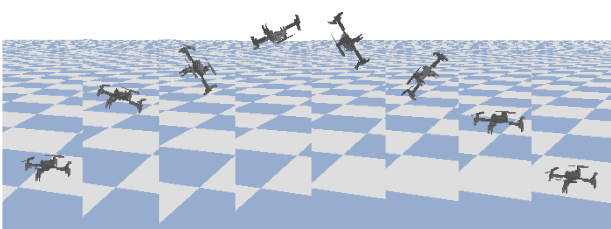
\includegraphics[width=.2\linewidth]{Fig/pics.png}
%\caption{Frames from the flip maneuver simulation video.}\label{fig:flipsimu}
%\end{figure}

\pagebreak
\subsection{Trajectory planning and geometric control}

The second control approach to perform a flip maneuver is trajectory planning and reference tracking with geometric control. Based on the results of the flip with open-loop control, the parameters of the reference pitch trajectory are chosen to $\alpha=20$~1/s, $\beta=0.45$~s, as illustrated in Figure \ref{fig:attref}. In the quadratic programming problem \eqref{eq:quadprog} we use the following parameters:
\begin{align}
    \mathcal{X}:\;\begin{bmatrix} x_- \\ x_+ \\ z_- \\ z_+ \end{bmatrix} =  \begin{bmatrix} -0.6 \\ 0 \\ -0.05 \\ 0.45 \end{bmatrix}\;\mathrm{m};\quad \mathcal{U}:\;F \in [0,0.64]\;\mathrm{N}; \quad T_s = 1/480\;\mathrm{s}.
\end{align}
The maximal collective thrust $F_\mathrm{max}=0.64$ N is from \cite{Forster}, and the position bounds are chosen such that the trajectory is feasible, and the quadcopter does not get too far from the initial point, for example we can express the available flying space here to avoid collision with walls or other objects. The duration of the flip is chosen to $T=0.9$~s, thus the number of simulation steps is $N=T/T_s=432$. The quadratic optimization problem is solved by the \verb+quadprog+ function of Matlab with negligible computation time. The result is the optimal control input and reference position sequence given in the discrete time instants.

The official Crazyflie 2.1 firmware has built-in trajectory evaluation algorithm for 7th degree polynomials\footnote{\url{https://www.bitcraze.io/documentation/repository/crazyflie-firmware/master/functional-areas/trajectory_formats/}}, therefore we fit such functions to the optimal position sequence, and use it as the reference for the flip maneuver. As both the $x$ and $z$ solution are smooth, the 7th degree polynomials can be fitted with almost zero error using the Curve Fitting Toolbox of Matlab\cite{matlabcurvefitting}.

The quadcopter follows the designed reference trajectory with geometric tracking control, based on the control law \eqref{eq:geomlaw} and error terms \eqref{eq:geomerrors}. The diagonal gain matrices were determined based on grid search and considering that the Mellinger controller \cite{mellinger2011} with a similar control law is part of the official Crazyflie 2.1 firmware\footnote{\url{https://www.bitcraze.io/documentation/repository/crazyflie-firmware/master/functional-areas/sensor-to-control/controllers/}}. The numerical values are as follows:
\begin{align*}
    K_r = \mathrm{diag}\left(\begin{bmatrix}
    0.5 \\ 0.5 \\ 1.25
    \end{bmatrix} \right);\quad K_v = \mathrm{diag}\left(\begin{bmatrix}
    0.2 \\ 0.2 \\ 0.8
    \end{bmatrix} \right);\quad K_R = 0.08 I_{33}; \quad K_\omega = 0.002 I_{33},
\end{align*}
 where the result of diag$(\cdot)$ is a $3\times 3$ matrix with the argument vector in the diagonal, and $I_{33}$ is the $3\times 3$ identity matrix.
 
 The simulation results of the trajectory planning and reference tracking with geometric control are displayed in Figure \ref{fig:geomsimu}. Similarly to the open-loop approach, the maneuver starts and ends at hovering, but in this case the stabilizing controller is also the geometric control with position and yaw setpoint. At the beginning of the maneuver, the controller is switched from yaw to pitch reference to follow the specified reference trajectory. The left plot illustrates the reference and simulated pose of the quadcopter during the backflip maneuver, and the right plot contains the trajectory of the pitch angle, angular velocity and collective thrust control input. The trajectory of both the angular velocity and the thrust input are smooth, opposed to the discontinuous angular acceleration and thrust of the open-loop control. In the discontinuities of the control input the unmodeled transient behaviour of the actuator dynamics can be significant, therefore the geometric control approach is more robust to such uncertainties compared to the open-loop method. 
 
\begin{figure}
    \centering
    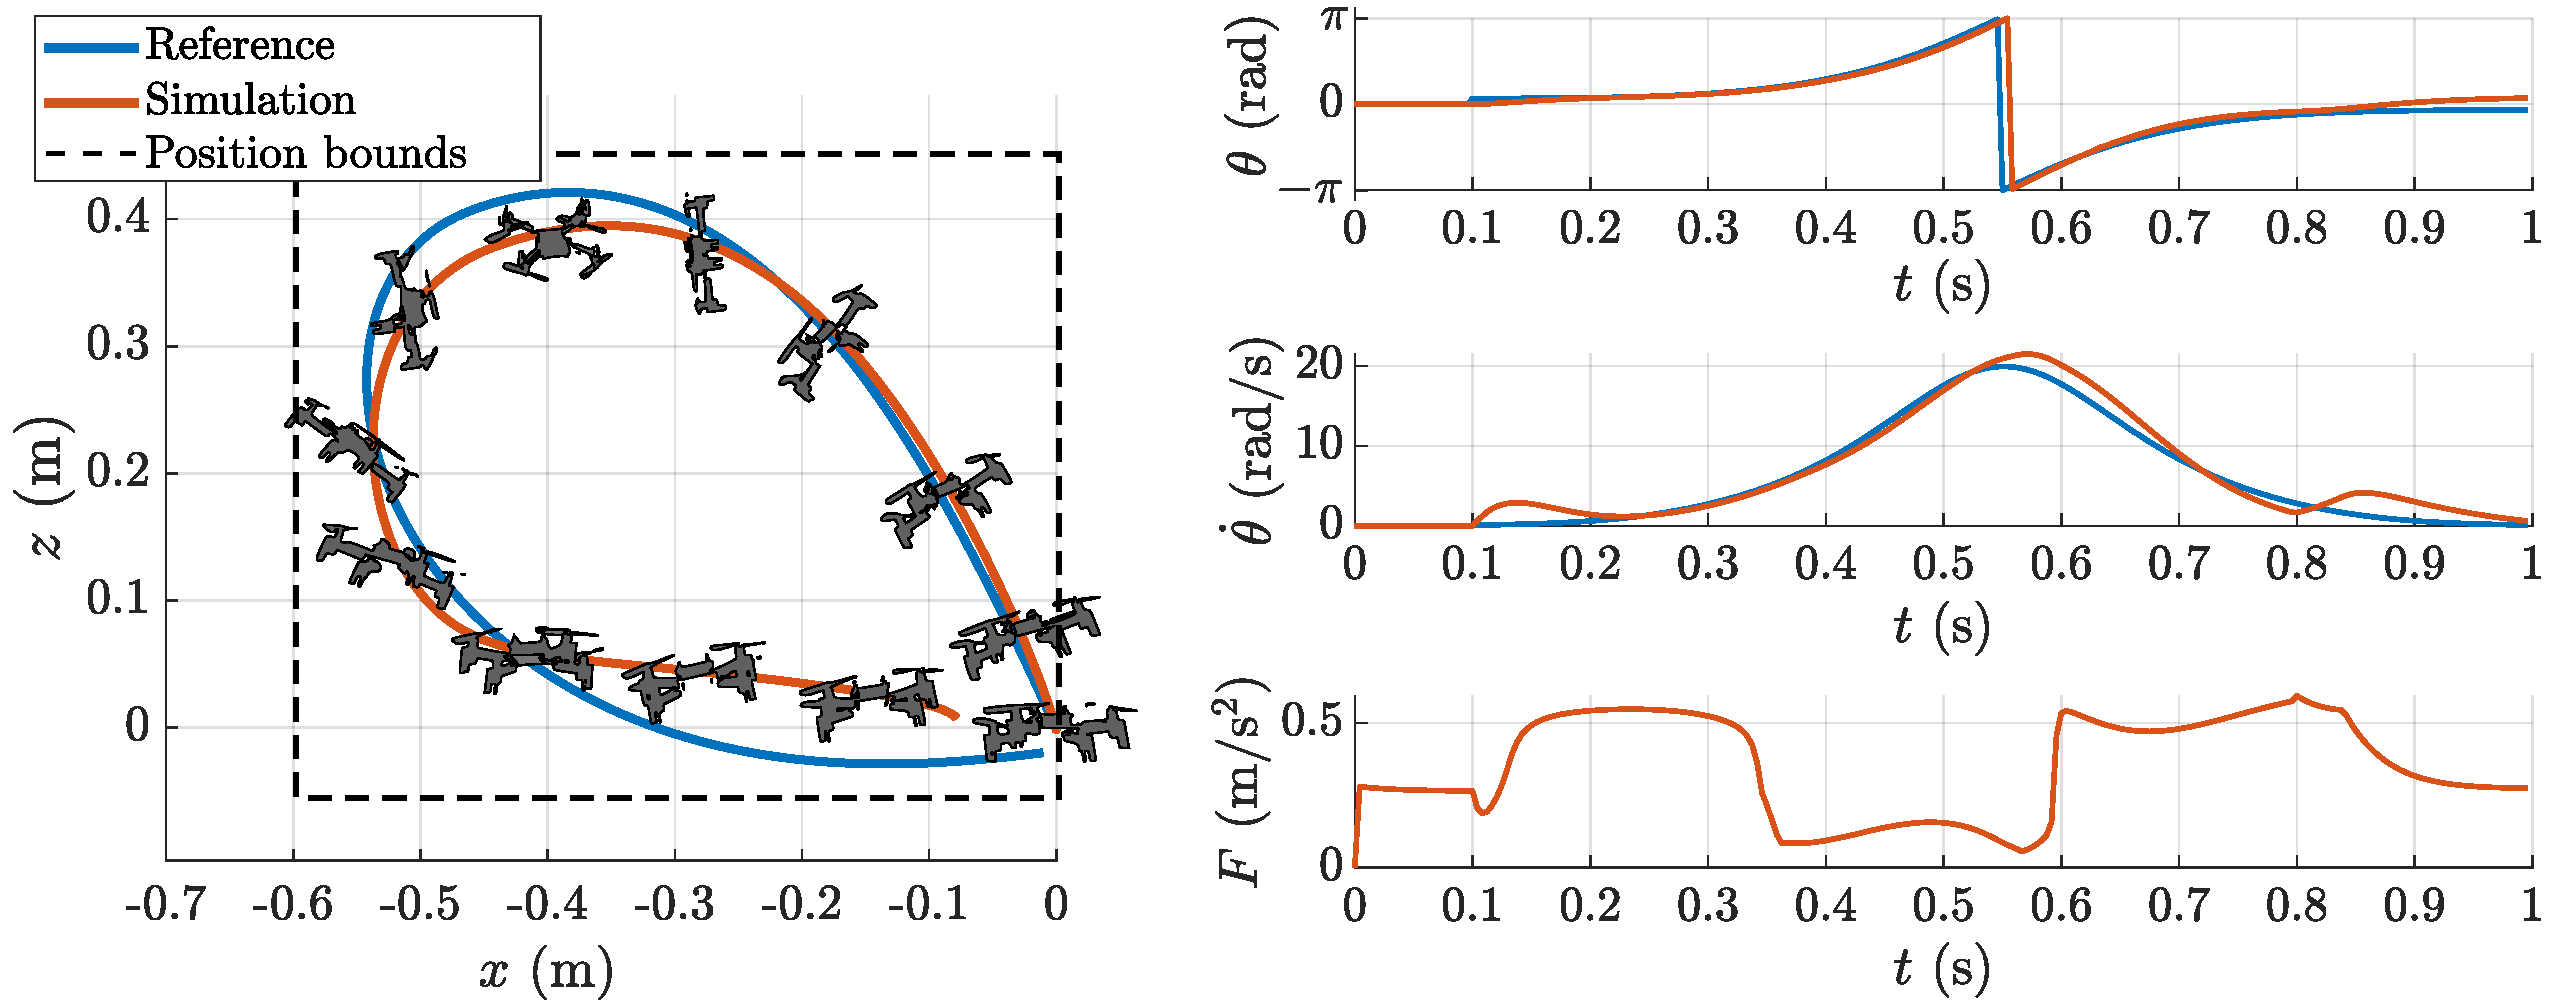
\includegraphics[width=\linewidth]{Fig/geomsimu.pdf}
    \caption[Backflipping simulation results with geometric control]{Backflipping simulation results with geometric control: position and attitude on the left, the pitch angle $\theta$, pitch angular velocity $\dot{\theta}$, and collective thrust $F$ on the right.}\label{fig:geomsimu}
    \end{figure}

\begin{figure}
    \centering
    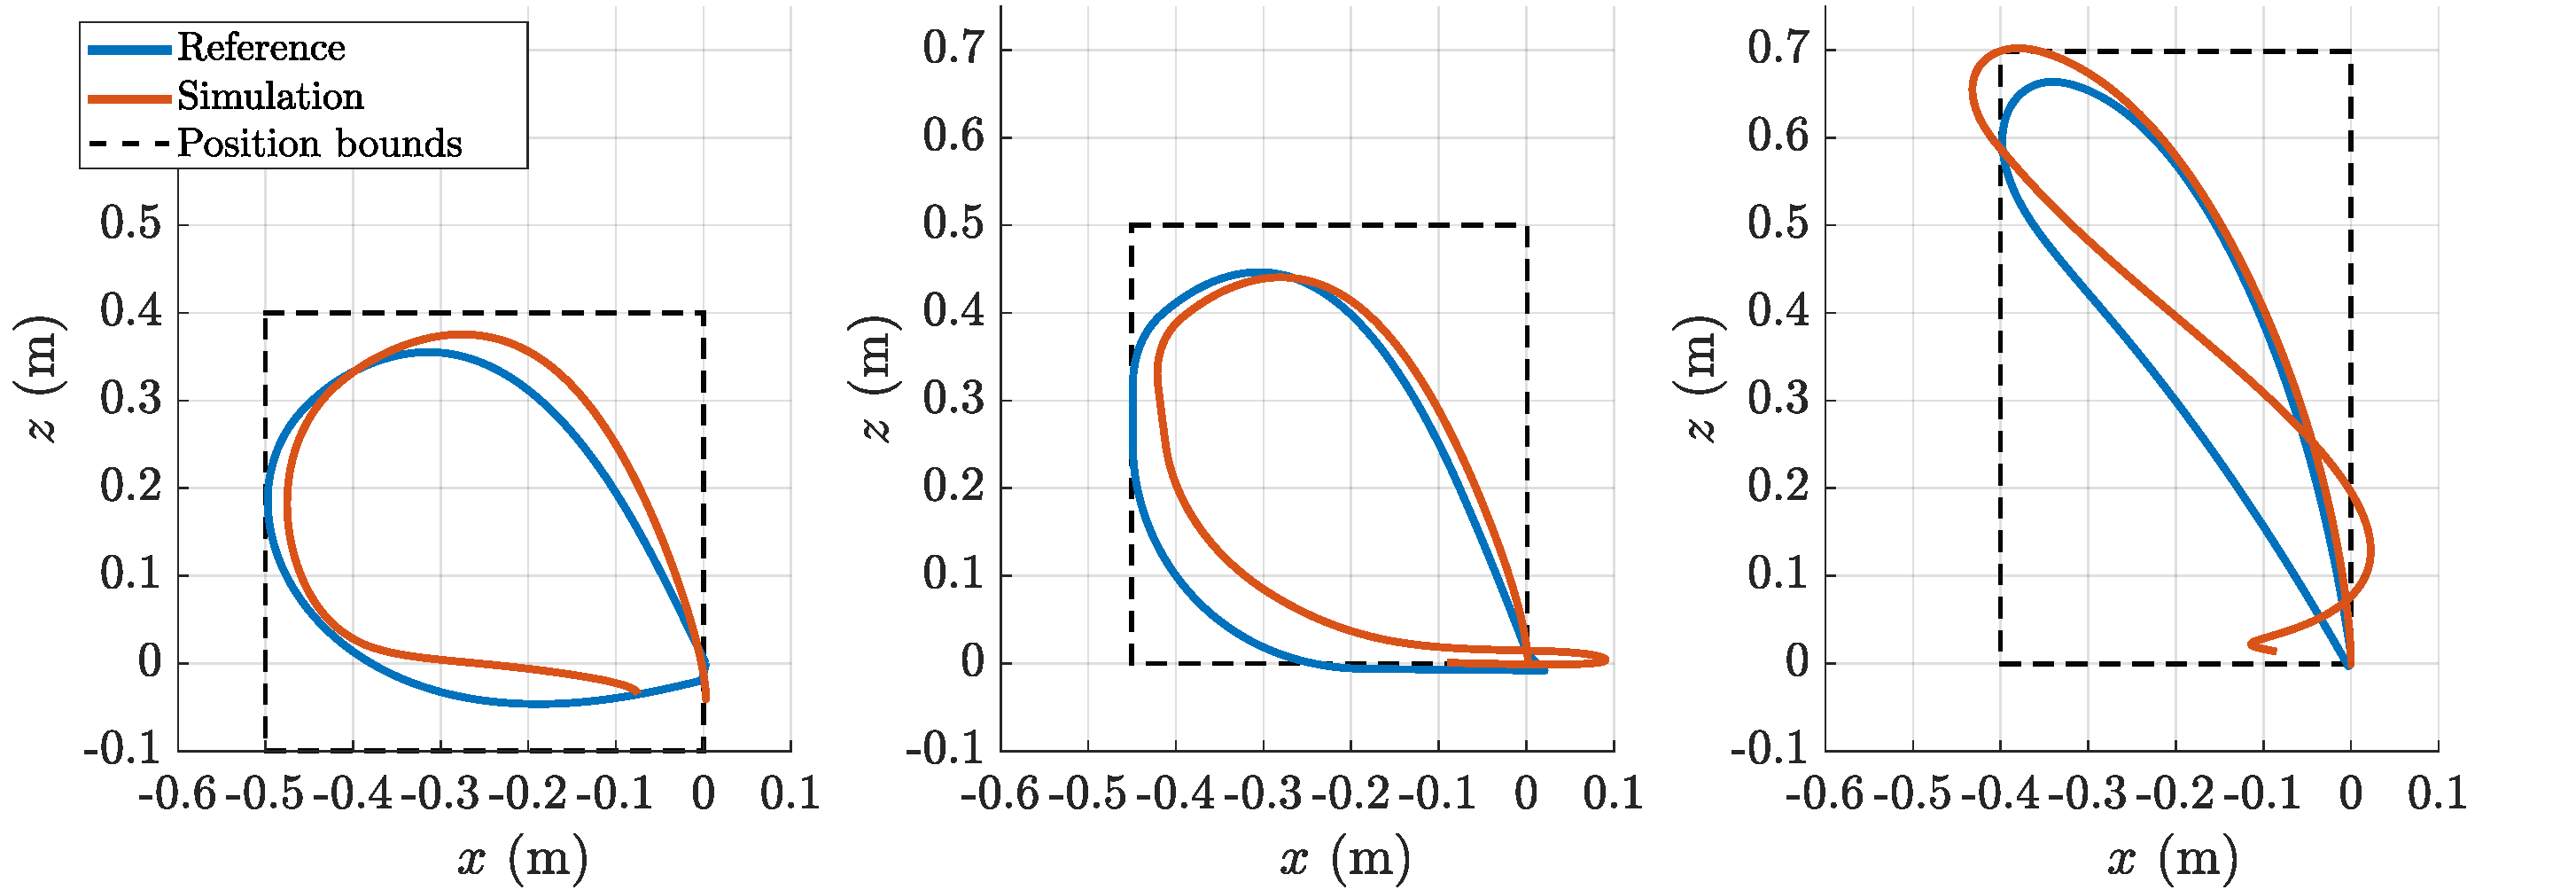
\includegraphics[width=\linewidth]{Fig/geomsimu2.pdf}
    \caption[Backflipping simulation results with geometric control: the effect of position constraints]{Backflipping simulation results with geometric control. The position reference constraint is different for each simulation, illustrated by the dashed lines.}\label{fig:geomsimu2}
\end{figure}
 
 It can be seen that the orientation reference tracking is more precise than the position. Fast and accurate attitude tracking is required to stabilize the quadcopter, however, the reference trajectory is designed with the assumption that the attitude equals to the reference at all times, therefore there are more significant errors in the position.
 
 

\section{Real-world implementation and experiments}\label{sec:exp}
In this section, real-world implementation of the two approaches to perform the backflip maneuver with the Crazyflie 2.1 drone, the experimental setup, and measurement results are presented. The experimental setup consists of the quadcopter with on-board sensors and microcontroller units (MCUs), the OptiTrack motion capture system, OptiTrack server, and ground control PC. The block diagram of the setup is displayed in Figure~\ref{fig:sys} with the direction and content of the information flow between the components.

\begin{figure}[b]
\centering
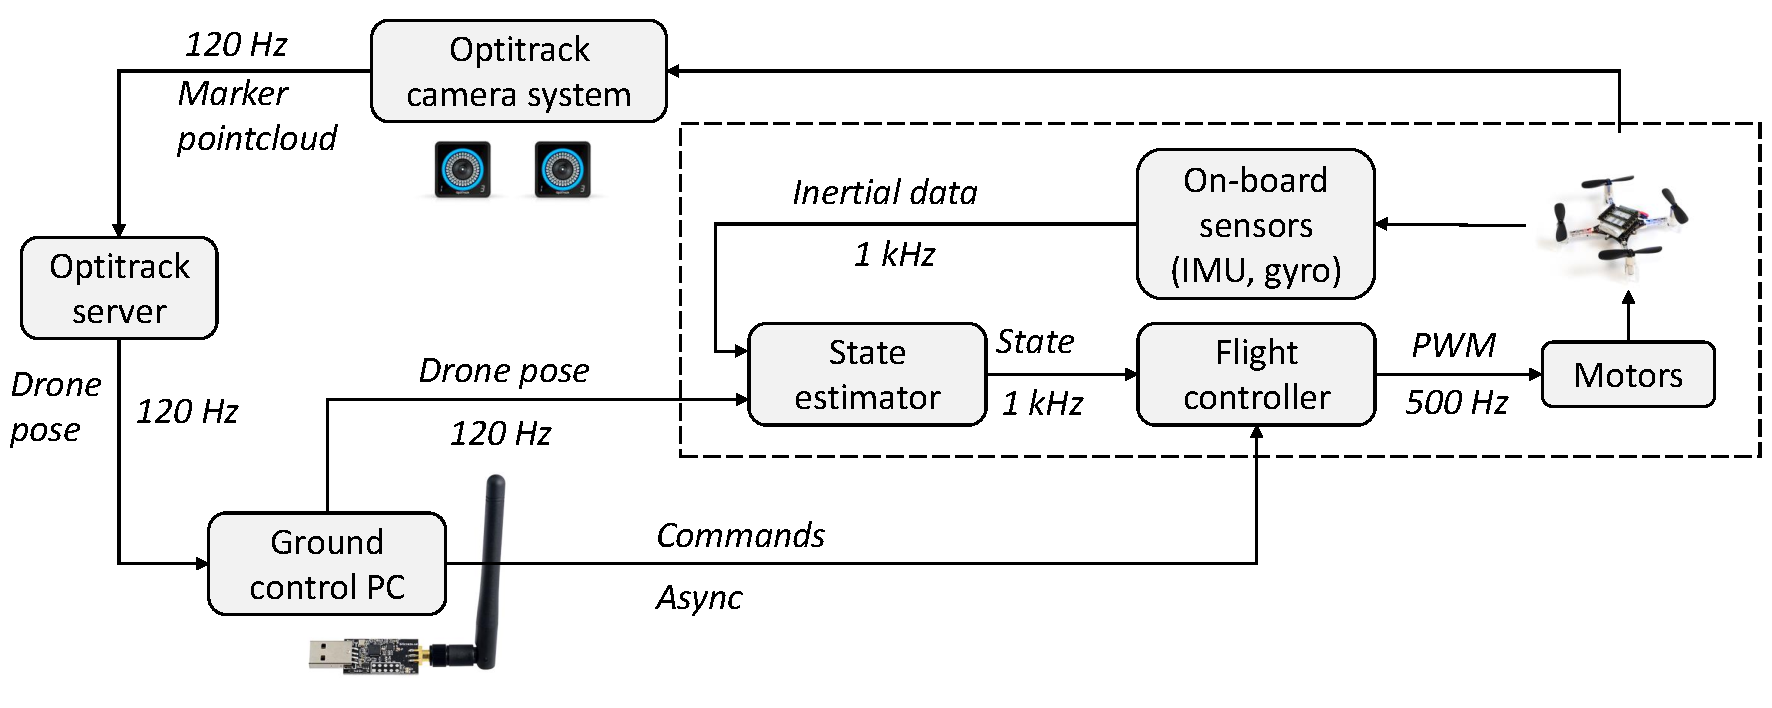
\includegraphics[width=.8\textwidth]{Fig/system.pdf}
\caption{Block diagram of the experimental setup: indoor quadcopter navigation with internal and external measurement system.}
\label{fig:sys}
\end{figure}

\subsection{The Bitcraze Crazyflie 2.1 drone}
This subsection presents an overview of the hardware and software of the Crazyflie 2.1 nano quadrotor, developed by the Swedish company Bitcraze AB. The vehicle is designed to be a development platform for research and education, therefore it is both fully open source and open hardware. Firstly the hardware specifications are summarized, and afterwards the structure of the firmware and control implementation possibilities are discussed.

\subsubsection{Hardware}

The quadcopter is an out-of-the-box device, the user only needs to assemble the parts. The central unit contains IMU sensors with accelerometer, gyroscope, magnetometer and barometer, and two microcontrollers: a STM32F405 for running the main application (e.g. state estimator, controller), and a nRF51822 for radio communication and power management. The four 4.2 V coreless BDC motors are connected to the central unit with plastic motor mounts. The propellers are fixed to the motor shafts using interference fit, and a 250 mAh LiPo battery is connected to the central unit to provide electric power. The drone weighs 28 grams, and the propeller-to-propeller distance is 92 millimeters.

Using the stock battery the flight time is 7 minutes without any external payloads. The maximum recommended payload is 15 grams including the extension decks which can be mounted to the drone. We only use one extension deck, on which the OptiTrack markers are mounted (see Fig. \ref{fig:hardware}), but there are several possibilities to extend the functionality and visual effects, for example the flow deck for optical flow measurement or the LED-ring deck.

The workstation PC communicates with the drone via the Crazyradio PA 2.4 GHz USB dongle. The radio communication makes it possible to update the firmware without a cable, and communicate with the quadrotor mid-flight, i.e. send external position data, update parameters, or log measurement data. The main parts of the hardware are displayed in Figure \ref{fig:hardware}.


\begin{figure}
\centering
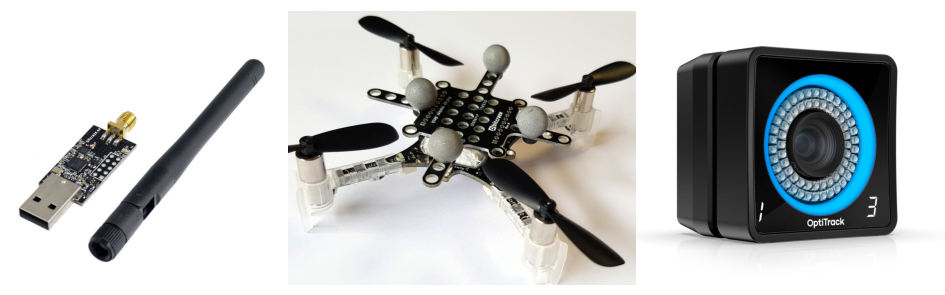
\includegraphics[scale=.6]{Fig/hardware.pdf}
\caption{The Crazyradio PA, Crazyflie 2.1 with motion capture markers, and an OptiTrack Prime 13 camera.}\label{fig:hardware}
\end{figure}

\subsubsection{Software}
The open-source software continuously developed by Bitcraze\footnote{\url{https://www.bitcraze.io/documentation/repository/}} includes the firmware, a Python client application and Python library with examples. In addition, we use the Crazyswarm platform \cite{crazyswarm} to easily handle the high-level control of multiple drones simultaneously, the OptiTrack measurement data, logging, and communication.

Out of all software components, we mostly use the firmware written in C language to implement our on-board controller, and the Python API for high-level commands and computation. The nRF51822 microcontroller manages the communication and power distribution, in which areas the default implementation is sufficient for us. However, the firmware of the STM32F405 contains the stabilizer unit responsible for handling high-level commands, state estimation and control input calculation. Two state estimators are implemented in the stock firmware of the Crazyflie: a complementary filter and extended Kalman filter. We use the latter, as it is more accurate for the fusion of internal and external sensor data.

There are three built-in controllers in the default firmware, a cascaded PID controller, the Mellinger controller \cite{mellinger2011}, and the  Incremental Nonlinear Dynamic Inversion (INDI) controller \cite{indi2015}. In this project, we use the PID controller for setpoint stabilization before and after the open-loop flip maneuver. Our own implementation of the geometric controller is responsible for backflipping with pitch reference, setpoint stabilization, and more complex, aggressive trajectory tracking.

%The structure of the cascaded PID controller is built as follows. The outermost loop is position control, which receives and handles the position or velocity input from the commander, running at 100 Hz. The next cascade is the attitude controller, which takes the error of the desired attitude as an input from the sensors, and outputs the desired attitude rate, running at 500 Hz. The innermost loop is the attitude rate controller, which also runs at 500 Hz. It receives the filtered output of the gyroscope rates, and outputs the collective thrust and the three torques in \eqref{eq:inputs} directly to the power distribution module.


% \begin{figure}
% \centering
% 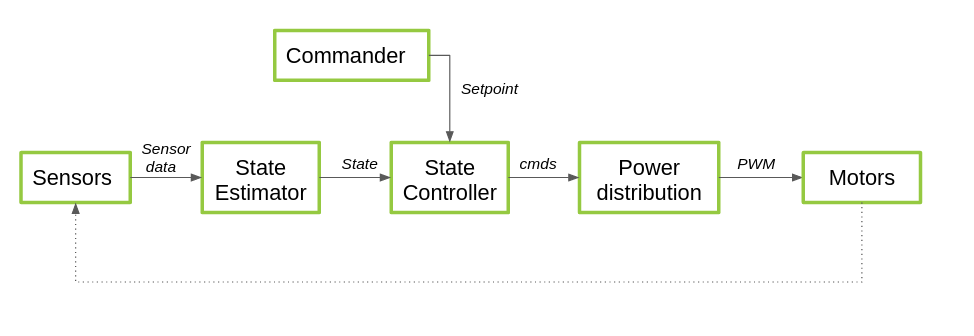
\includegraphics[width=\textwidth]{Fig/sensors_to_motors.png}
% \caption{Structure of the stabilizer module.}
% \label{fig:stab}
% \end{figure}



%\begin{table}[!h]
%\centering
%\begin{tabular}{l|c|c}
%mass & $m$ & 28 g\\
%\hline
%prop-to-prop length &$ l$ & 92 mm\\
%\hline

%\end{tabular}
%\caption{Physical parameters of the Crazyflie 2.1}
%\end{table}

\subsection{OptiTrack motion capture system}
At SZTAKI AIMotion Lab, we use OptiTrack for the real-time pose measurement of the drones which is a high precision motion capture system with submillimeter resolution. The system includes six Prime 13 infrared cameras sending the position information of specific markers at 120 Hz. Using the Motive software of OptiTrack, we can define rigid bodies with unique identifiers (both drones and obstacles), and broadcast their position and orientation information directly through local network.

Although OptiTrack is a very precise and efficient measurement device, sometimes it is not easy to arrange the markers on the drone such that at least four cameras see them at all times, especially during the flip maneuver. In these situations, the state estimator of the drone automatically switches to use only the information of the inertial measurement unit, which is sufficient for hovering and attitude stabilization.


\begin{figure}
\centering
\setlength{\fboxsep}{0pt}%
\setlength{\fboxrule}{1pt}%
\fbox{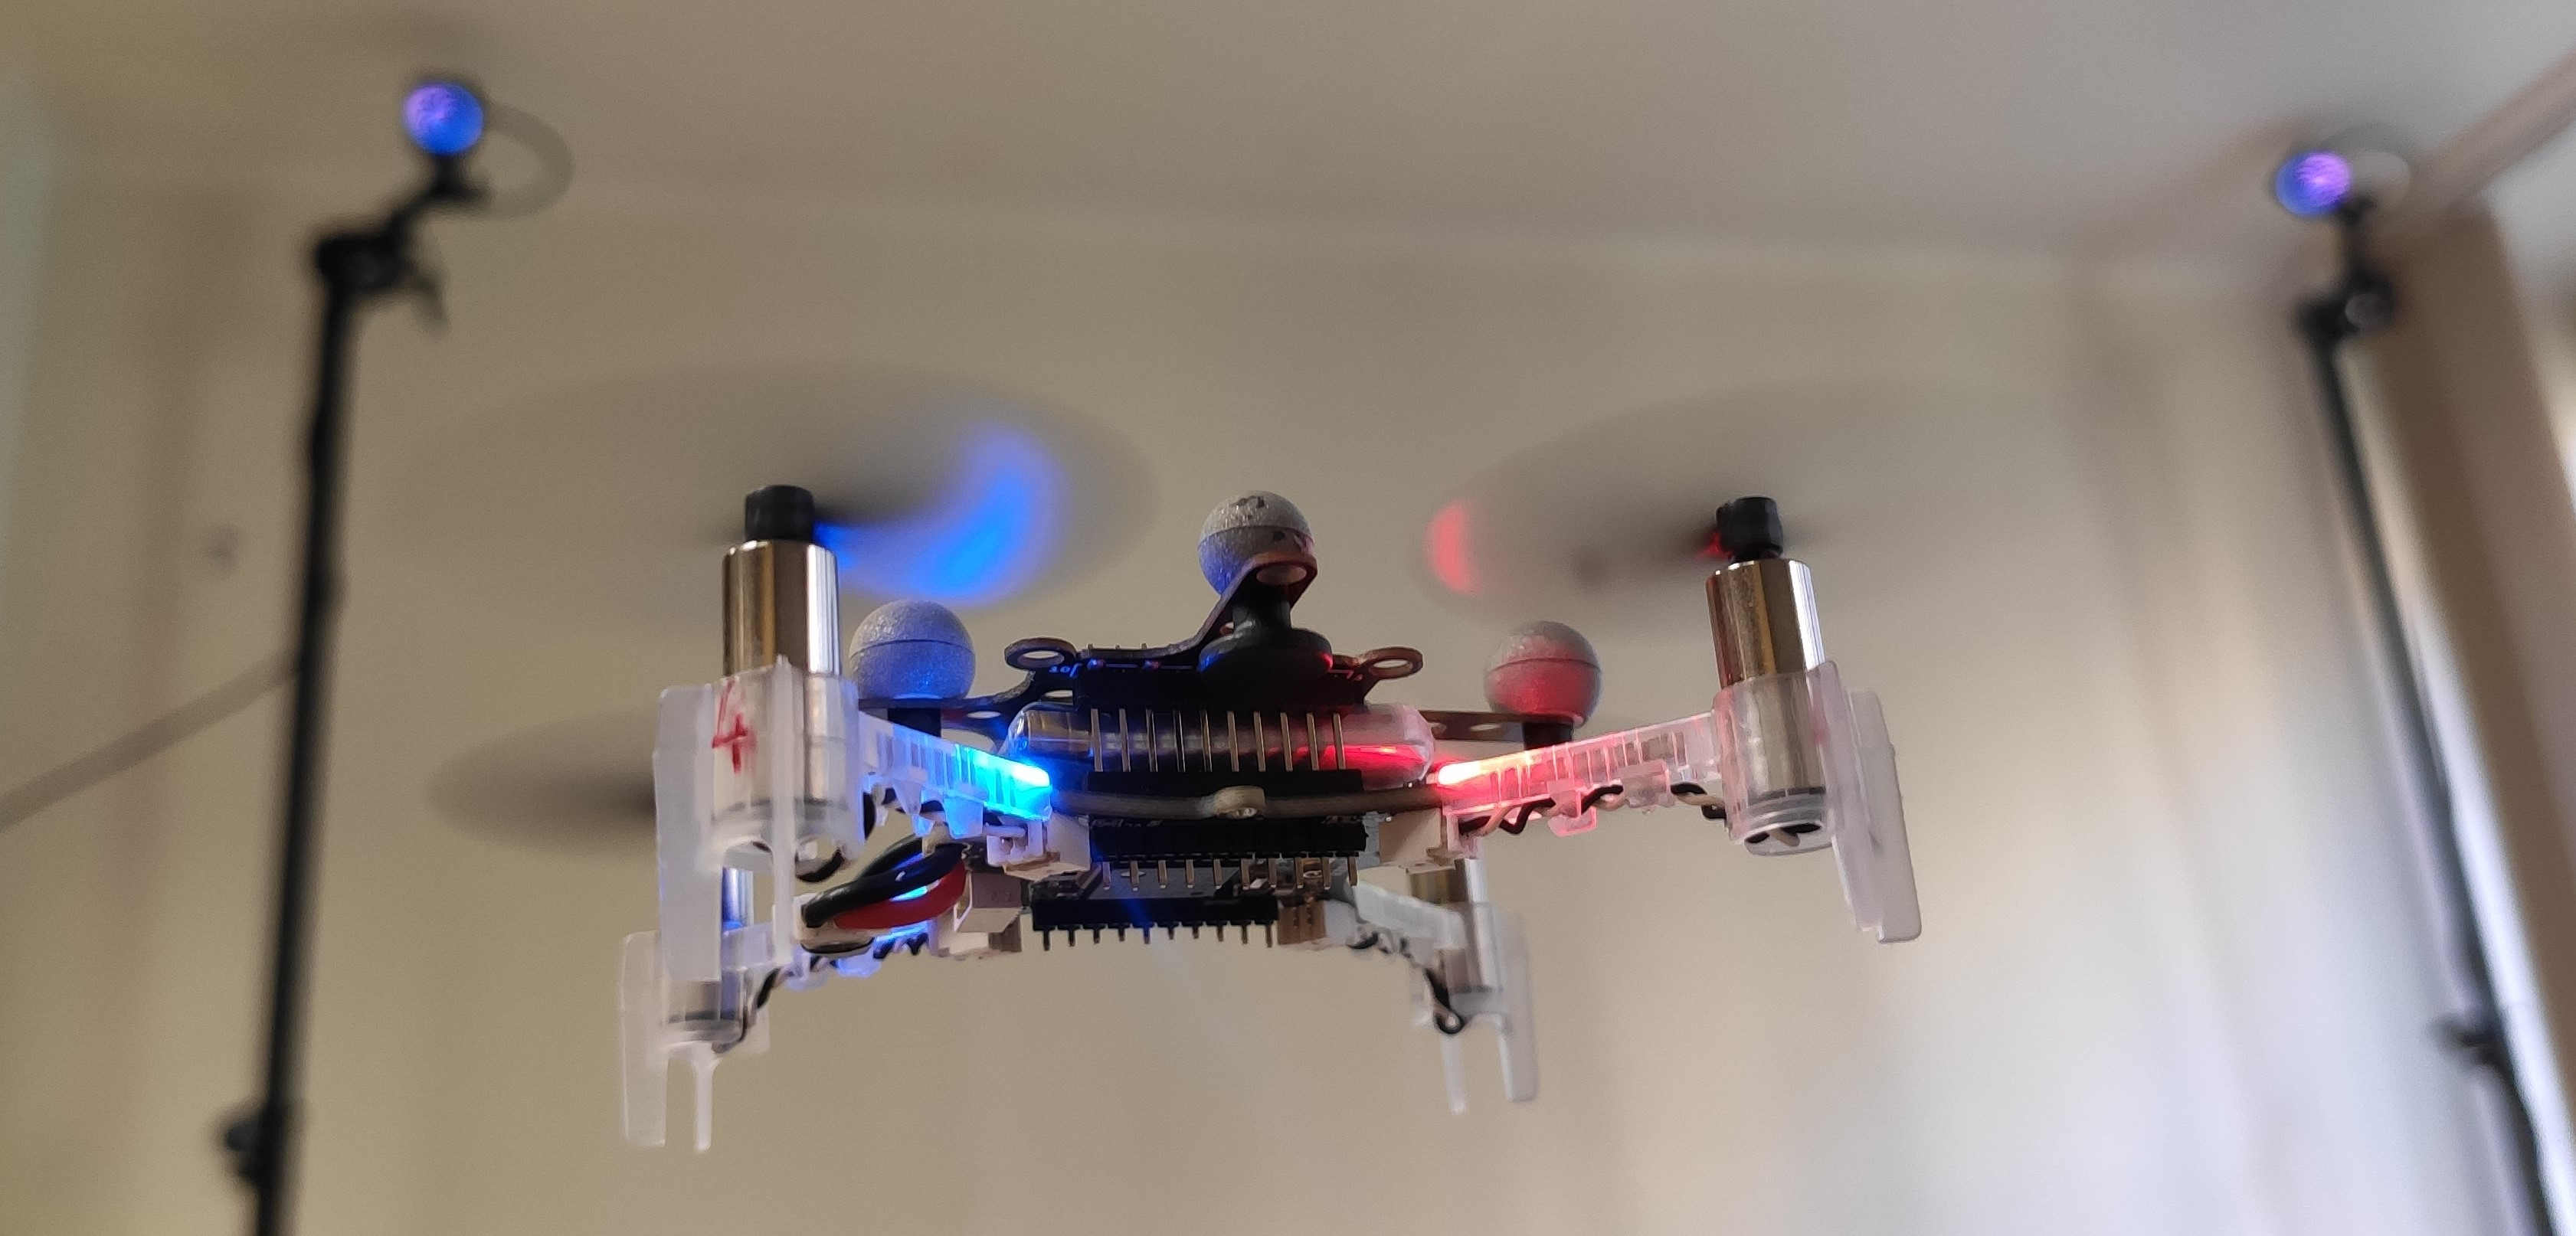
\includegraphics[width=.6\textwidth]{Fig/dronepic.jpg}}
\caption{Experimental setup for the presented measurement results: 2 OptiTrack Prime 13 infrared cameras and a Crazyflie 2.1 quadcopter with reflective markers.}
\end{figure}

\subsection{Backflip maneuver implementation}\label{sec:implementation}
In the Crazyswarm framework (running on the workstation PC) there are built-in examples for the high-level control of the quadcopter: for example it is enough to call the \verb+takeOff()+, \verb+goTo()+, and \verb+land()+ methods from a script to take off, hover for a specified duration, go to a given point in space, and land -- these commands are sent to the on-board microcontroller through a ROS C++ layer and the Crazyradio PA. In the \verb+.launch+ file of ROS, the user can specify the initial position of the drone, the controller type, state estimator type, logging variables, and other properties. The firmware parameters can be modified mid-flight, for example to adjust controller gains, or switch between controller types.

Our own implementation is a modified version of Crazyswarm, available at the GitHub repository \verb+TDK2021/real_quadcopter/crazyswarm+\footnote{\url{https://github.com/antalpeter1999/TDK2021}}. Our main contributions are in the controller of the firmware (open-loop and geometric control), and in the Python API for high-level commands, and simultaneous control of multiple drones.

The high-level script to perform a backflip maneuver is quite simple, because all control algorithms are implemented on-board. However, we need to build and flash the firmware of the quadcopter MCU after every change in the source code, therefore parameter setting and execution of high-level tasks is easier using Python scripts. The steps of the high-level script to perform the backflip are illustrated in Algorithm \ref{alg:hl}.

\begin{algorithm}
  \caption{High-level script executed on the ground control PC}
  \label{alg:hl}
  \begin{algorithmic}[1]
    \State Send parameters to the Crazyflie: controller type (open-loop or geometric), trajectory information, controller gains
    \State Take off and hover at the initial point of the flip
    \State Start the flip maneuver, and wait until it is over
    \State Land
  \end{algorithmic}
  \end{algorithm}

The evaluation of the open-loop control law, i.e. the calculation of control inputs from the current time has small computational cost, therefore it is practical to be implemented on-board. The implementation is detailed in Algorithm \ref{alg:open}, the maneuver is triggered from the ground station with a high-level command, it is executed automatically, and the quadcopter ends in hovering mode afterwards.
%In our implementation of this controller, the user only needs to set the value of \verb+isFlipControl+ variable to true, the quadcopter immediately starts the flip maneuver, and then automatically switches back to PID control. The parameters of the maneuver are sent to the drone before taking off (at the beginning of the high-level script). %The flip control policy is implemented within the innermost loop of the PID control code, therefore it runs at 500 Hz.
\begin{algorithm}
  \caption{Open-loop control on-board implementation}
  \label{alg:open}
  \begin{algorithmic}[1]
    \State Hover with PID control, wait for ground station command to start the backflip
    \State Lift with PID control to gain momentum
      \While {the flip is not over}
      \State Decide in which section we are (out of the 5 in Fig. \ref{fig:sections})
      \State Apply the control input of the current section based on \eqref{eq:openinp}
    \EndWhile
    \State Stabilize the quadcopter with PID control
    \State Get back to initial position
  \end{algorithmic}
  \end{algorithm}

The second control approach, i.e. reference trajectory tracking with geometric control is also implemented on-board. The coefficients of the designed trajectory represented by 7th degree polynomials, and the corresponding time duration are saved to a csv file after the simulations. In the Python API, it is loaded and sent to the Crazyflie with the tuned controller gains, before taking off. The on-board implementation of the control approach is detailed in Algorithm~\ref{alg:geom}. Similarly to the open-loop approach, the command to start the maneuver comes from the ground station, and then the backflip is performed automatically.
\begin{algorithm}
  \caption{Geometric tracking control on-board implementation}
  \label{alg:geom}
  \begin{algorithmic}[1]
    \State Hover with geometric control, wait for ground station command to start the backflip
    \State Lift with geometric control to gain momentum
      \While {the flip is not over}
      \State Get the current state from the state estimator module
      \State Get the setpoint by evaluating the reference trajectory
      \State Calculate the control inputs from the control law \eqref{eq:geomlaw}
      \State Apply the control inputs to the motors
    \EndWhile
    \State Stabilize the quadcopter with geometric control
    \State Get back to initial position
  \end{algorithmic}
  \end{algorithm}


 %When the user wants to start the backflip maneuver, similarly to the open-loop method, only needs to set the value of \verb+isFlipControl+ to true. The on-board algorithm then starts executing the previously saved trajectory, switches to pitch reference from yaw reference, and switches back after the maneuver is over. 

%A big advantage of the on-board control is that the maneuver can be performed by multiple quadcopters simultaneously without any problems coming from communication delays and lost packages between the ground control PC and the drone microcontroller.

\subsection{Experimental results}

Experiments to perform the backflip maneuver started with the open-loop method. Firstly, we used the optimal parameter set from \eqref{eq:optparam}, but due to the differences of the simulation model and the real quadcopter dynamics, the drone almost performed a double flip with these parameters, and the stabilization was not successful at the end of the maneuver. After realizing the differences between the measurements and the simulations, we manually tuned the parameters so that the flip is executed with minimal final state error. The refined experimental parameter set is
\begin{align*}
    P^\mathrm{exp} = \begin{bmatrix}
U_1^\mathrm{exp} & t_1^\mathrm{exp} & t_3^\mathrm{exp} & U_5^\mathrm{exp}& t_5^\mathrm{exp}
\end{bmatrix} ^\top =  \begin{bmatrix}
14.29 & 0.2 & 0 & 14.29 & 0.075
\end{bmatrix}^\top.
\end{align*}
The measurement results are displayed in Figure \ref{fig:openmeas}, showing the trajectory of the position and orientation during the maneuver. It is important to note that an additional lift phase is added to the implementation to gain enough vertical velocity and height, because the quadcopter falls a significant distance in the recovery phase. During the additional lift phase the PID controller is used to achieve exact vertical lifting and horizontal orientation.

Figure \ref{fig:openmeas} shows that the flip is executed with almost zero final error in the pitch, and also quite small position error. 

The experimental results of the backflipping with geometric control are displayed in Figure~\ref{fig:geommeas}. The most important part of reference tracking is the pitch angle $\theta$, because a fast, stable and accurate attitude tracking is required to perform the flip maneuver, and recover successfully. As it is shown on the upright plot of the measurement results, the pitch is very close to the reference. 

However, the error of the position tracking is significantly higher during the maneuver, both in $x$ and $z$ directions. There are many possible reasons of the high positioning error, the following are the most likely. Firstly, we assume at the trajectory design that the orientation is equal to the reference at all time steps, which is not far from reality, but there is always a non-zero attitude tracking error. It was another assumption of trajectory design that the derivative of the control input can be arbitrarily large, the optimization problem formulation does not include an error term or constraint for this variable. However, when the quadcopter is upside down, a near-minimal collective thrust is required, and shortly after a near-maximal thrust to recover and follow the reference, as it is illustrated in Figure \ref{fig:geommeas}. Small DC motors are usually modelled as first order systems with a small time constant, but here the transient can be significant, the motor needs time to build the thrust of the propellers. The third possible explanation is also connected to model uncertainty. The modelling of aerodynamic effects such as blade flapping, induced drag or downwash \cite{quad_model} are very complex, therefore we exclude these terms from the dynamic model, however, they can have a negative effect on the performance of the feedback controller when performing the backflip maneuver.

\begin{figure}
\centering
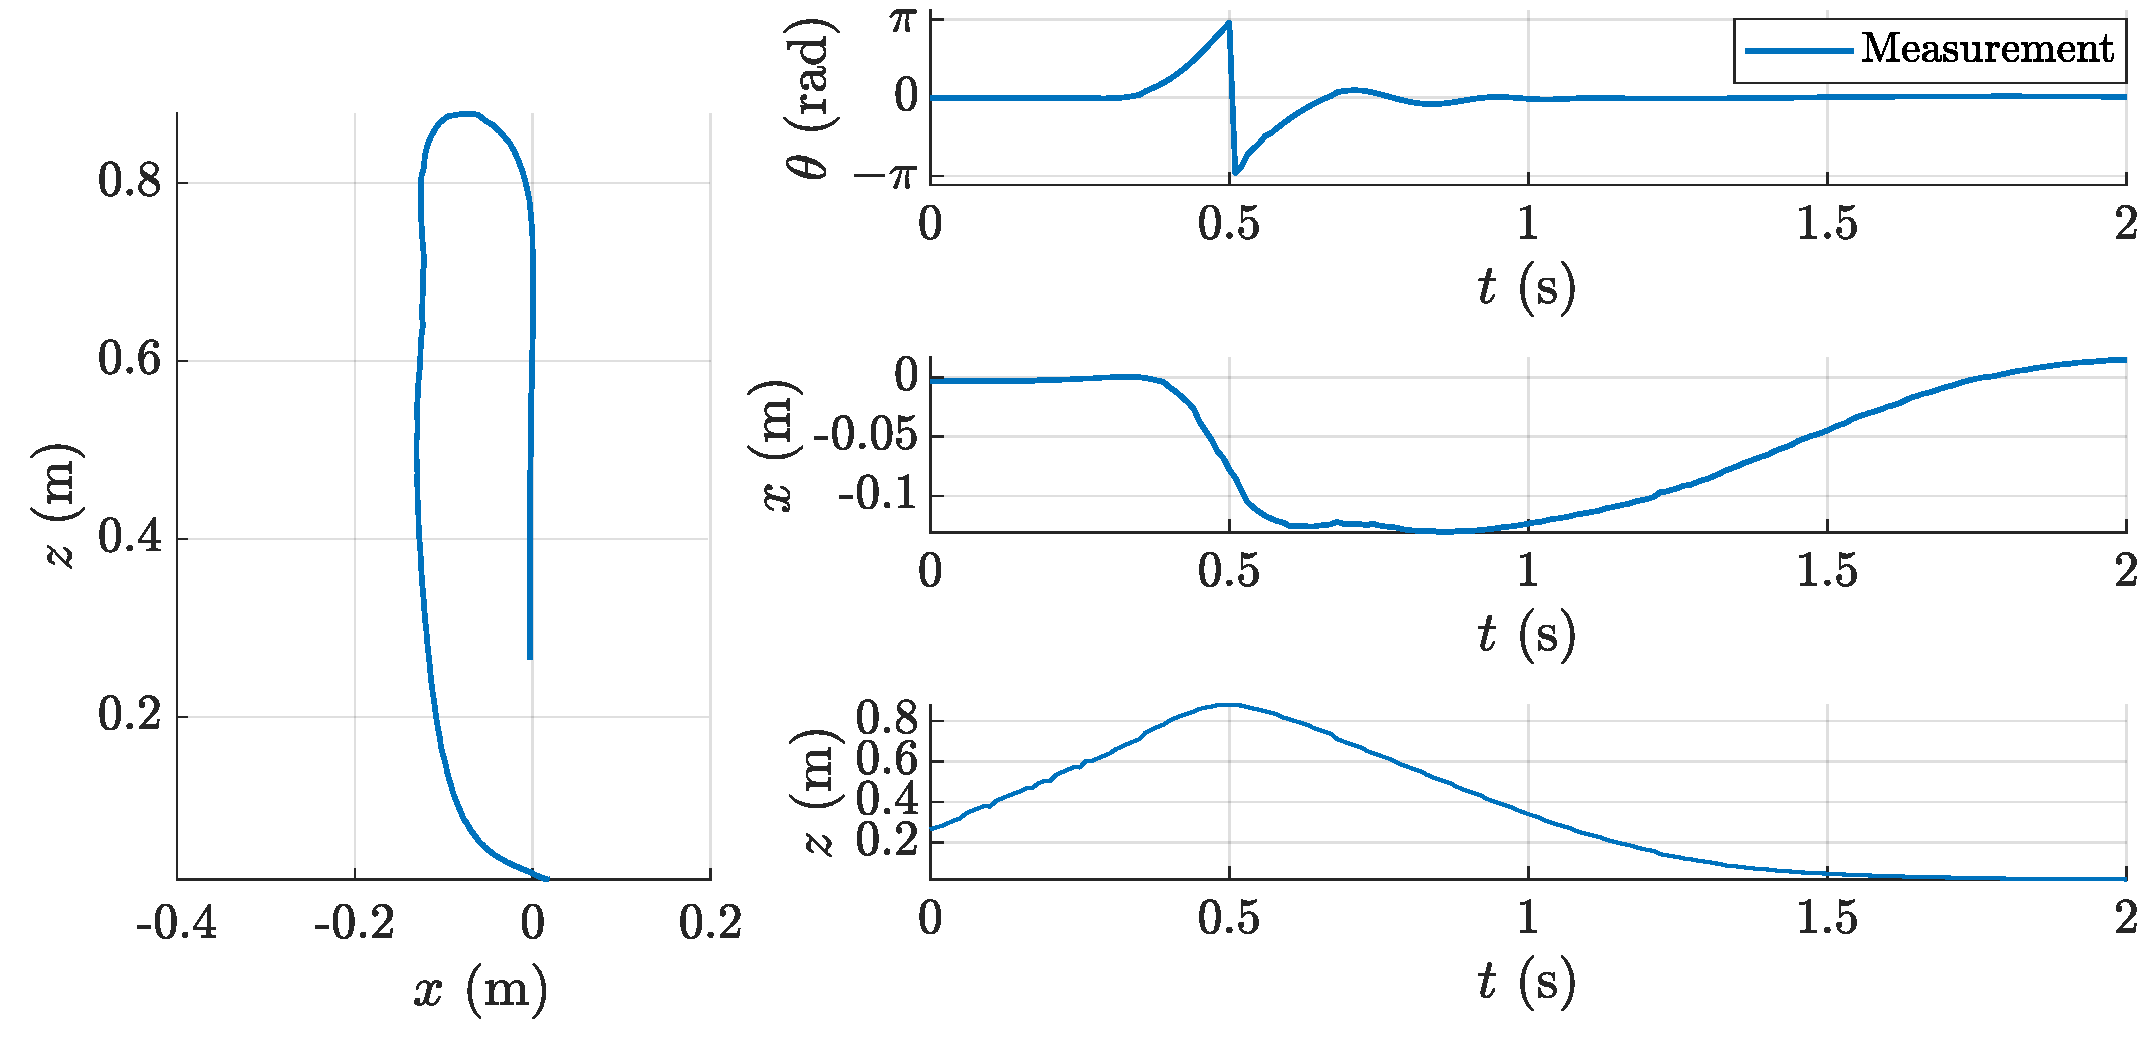
\includegraphics[width=\linewidth]{Fig/openmeast.pdf}
\caption{Backflipping measurement results with open-loop control.}\label{fig:openmeas}
\end{figure}

\begin{figure}
\centering
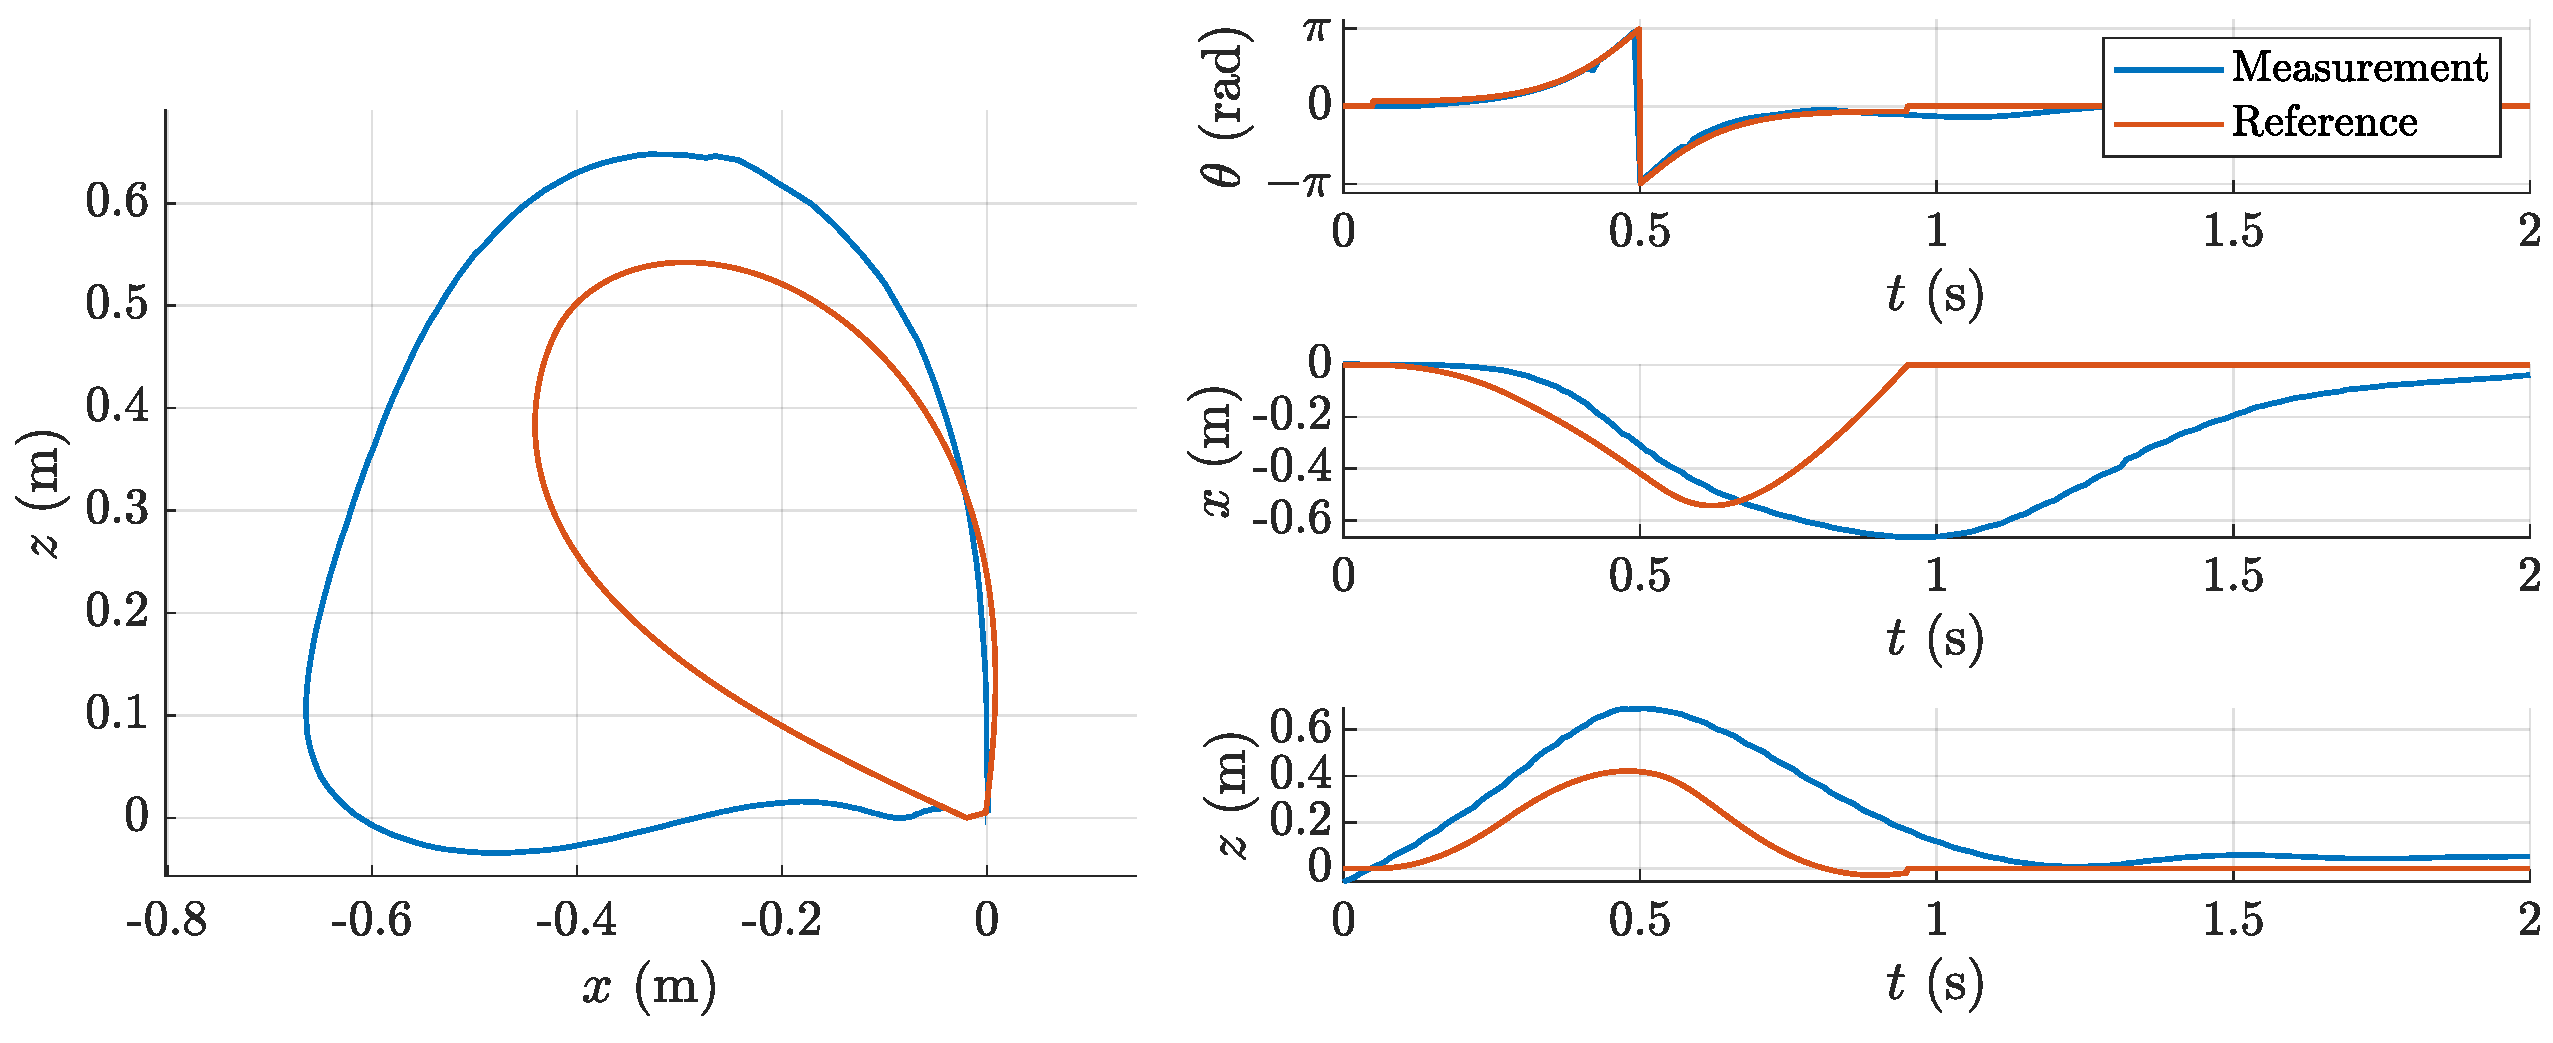
\includegraphics[width=\linewidth]{Fig/geommeast2.pdf}
\caption{Backflipping measurement results with geometric control.}\label{fig:geommeas}
\end{figure}

\begin{figure}
\setlength{\fboxsep}{0pt}%
\setlength{\fboxrule}{1pt}
\centering
\begin{subfigure}{.45\textwidth}
  \centering
  \fbox{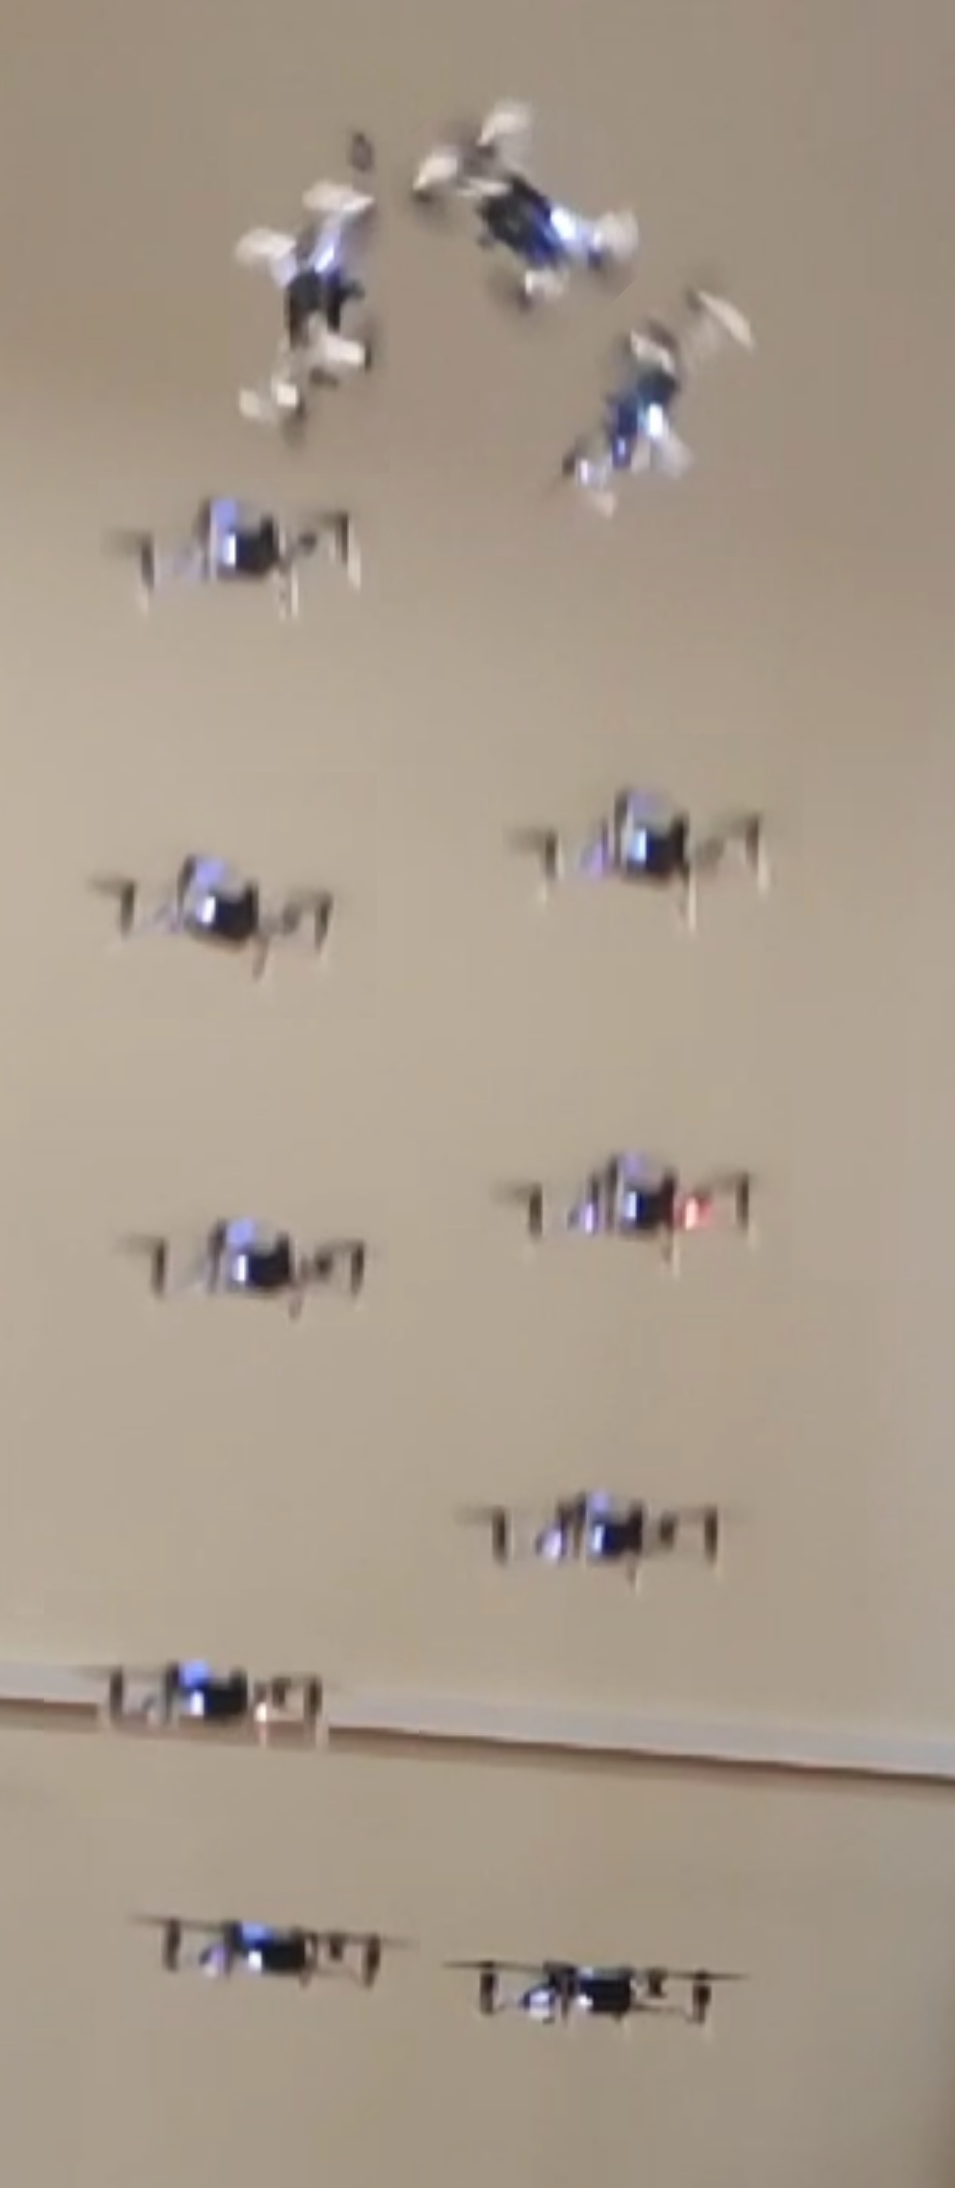
\includegraphics[height=6cm]{Fig/opencomp.png}}
  \caption{Optimization-based open-loop control, the trajectory is displayed in Fig. \ref{fig:openmeas}}
  \label{fig:sub1}
\end{subfigure}%
\hspace{1cm}
\begin{subfigure}{.45\textwidth}
  \centering
  \fbox{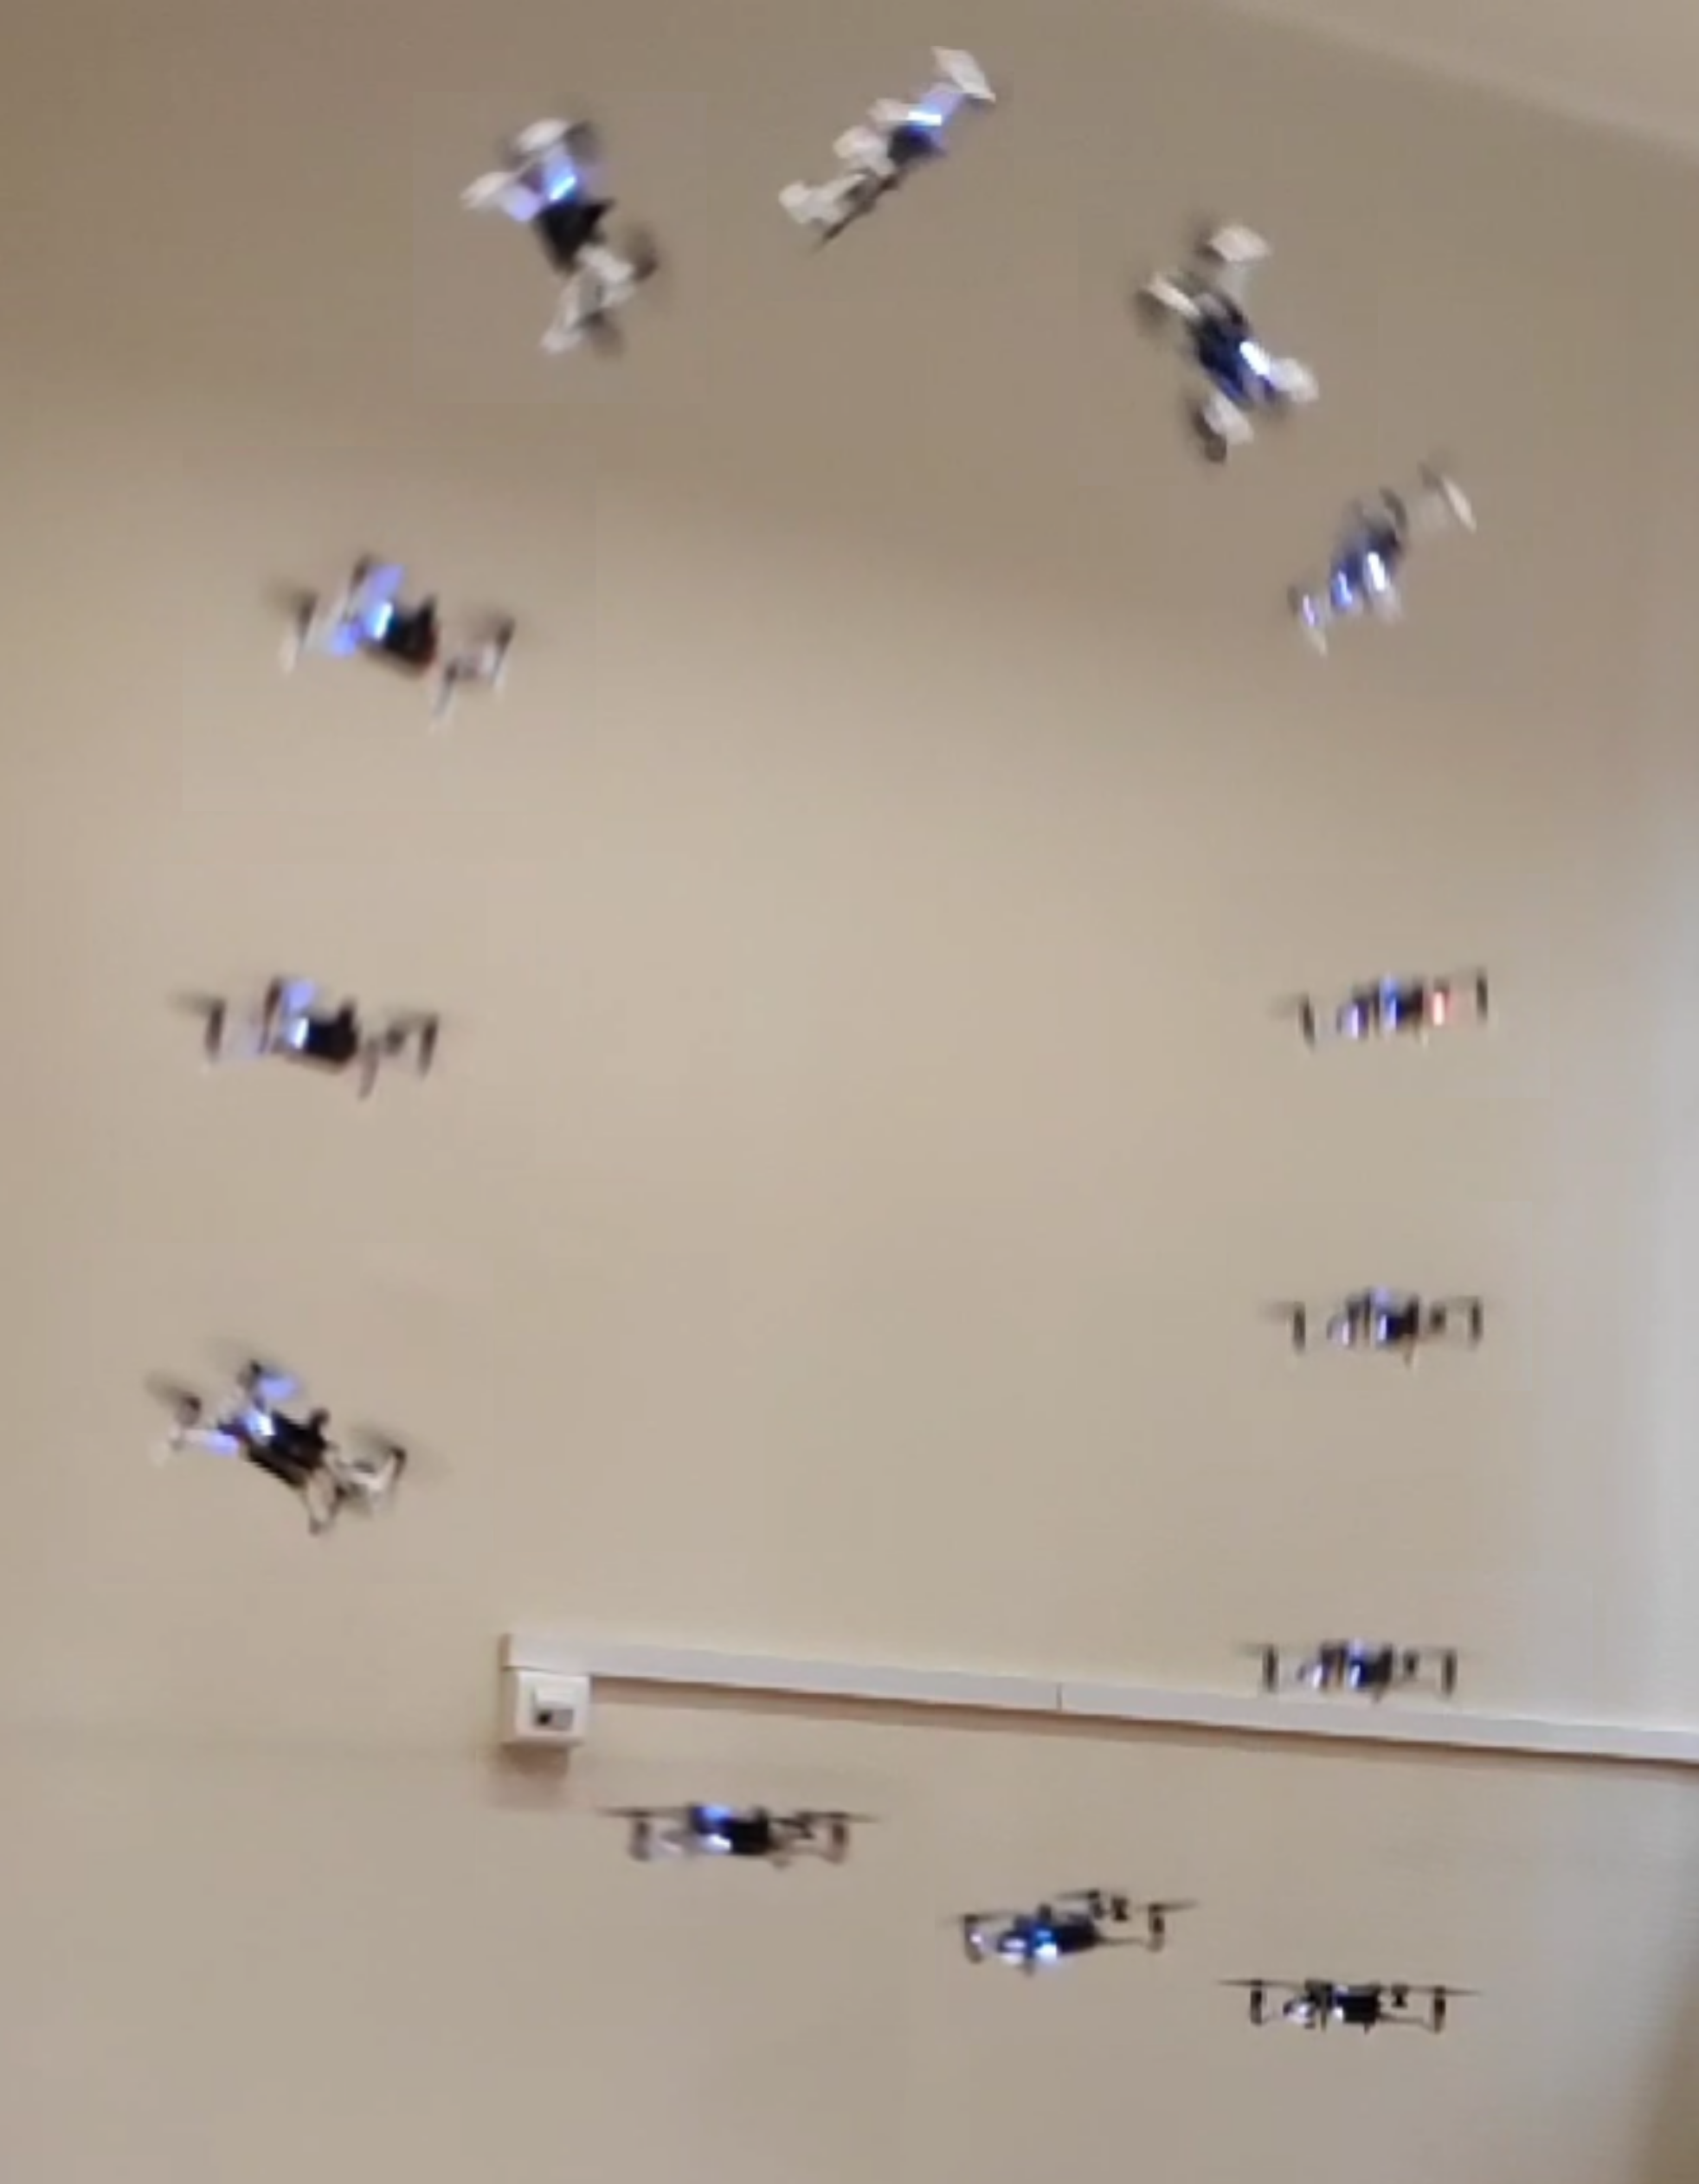
\includegraphics[height=6cm]{Fig/geomcomp.png}}
  \caption{Geometric reference tracking control, the trajectory is displayed in Fig. \ref{fig:geommeas}}
  \label{fig:sub2}
\end{subfigure}
\caption{Composite images of the measurement results with both proposed control methods. A video of the measurements is available at \textit{\textbf{TODO}}}
\label{fig:test}
\end{figure}

\subsection{Robustness and scalability for multiple drones}
The presented measurement results are satisfactory for both control methods, the quadcopter performed a backflip maneuver successfully. However, the open-loop approach is very sensitive to parameter uncertainties, therefore it needs specific tuning for each Crazyflie. Moreover, it is also sensitive to initial conditions, because the open-loop control input is the same even if there is a nonzero angle or displacement at the starting point. Hence the quality of the maneuver often varies even with the manually refined parameters. Due to the inconsistency of the performance, we could not apply the open-loop control for simultaneous flip with multiple drones.

However, geometric tracking control overcomes the problematics caused by parameter uncertainties using feedback, providing a highly robust and consistent performance for the backflip maneuver. Utilizing the robustness of the control approach, the maneuver has been implemented for simultaneous backflipping with three drones. A video of the acrobatic maneuver is available at \textbf{\textit{TODO}}. The implementation of the simultaneous flip differs from the single maneuver discussed in Section \ref{sec:implementation} only in the high-level script. The trajectory of each drone during the maneuver is evaluated relatively to their initial position and orientation, making it easy to extend the single flip implementation. % In the high-level script we send each drone to their initial pose, and send the command to start the flip. Afterwards, the quadcopters hover at the initial pose and wait for the next command, for example to land.

The scalability of the proposed control algorithms for other types of quadcopters (e.g. medium or large-sized) is out of the scope of this work, however, the possibilities are briefly discussed in the followings. The open-loop method is applied in \cite{LSICRA2010} to a medium-sized drone successfully, therefore we are convinced that our modified version could also be applied to other types. Geometric control is even more general than the open-loop approach, it is applied not only for different types of quadcopters \cite{turpinkumar2011}, but also for other autonomous systems, such as robotic manipulators \cite{bullo2004}.

\section{Conclusions and future work}
The aim of this work is to develop and implement control algorithms for performing a backflip maneuver with miniature quadcopters. A thorough literature survey has been conducted about the mathematical modelling of quadcopter dynamics, control approaches for aggressive maneuvers, and specifically for backflipping. The first proposed control method is an open-loop strategy based on the optimization of a parametric motion primitive sequence. We have interpreted the work of \cite{LSICRA2010}, and extended it with Bayesian optimization which we have found more suitable for parameter optimization. The second proposed strategy for backflipping is trajectory design and geometric feedback control for reference trajectory tracking. The nonlinear geometric control is part of the work in \cite{lelemc2010}, providing an almost globally stable control law on $SE(3)$. We have used basic assumptions from the open-loop approach as well (e.g. duration of the maneuver) to define a reference trajectory for the attitude of the quadcopter, represented in unit quaternions. The attitude reference has been used to design the reference position trajectory, computed as the solution of a constrained quadratic optimization problem on the discrete time model of the drone. The trajectory design is computationally efficient, flexible, and most importantly general, therefore it can be used to learn other complex maneuvers in a similar framing in the future.

After the theoretical foundation of the mathematical model and control approaches, we implemented the maneuver in simulation, using the parameters of the Bitcraze Crazyflie 2.1 quadcopter. The parameter optimization of the open-loop approach proved to be successful, the drone has learnt to perform the flip with good performance. The trajectory design for the second control method has been implemented in Matlab, and the geometric control in the same Python framework as the open-loop approach. With the proper tuning of geometric control gains, simulations has shown accurate trajectory tracking both for the position and orientation of the quadcopter, performing the backflip maneuver with small errors.
%The control algorithms run on-board, therefore they are executed with high frequency, running at $~500$ Hz. An external motion capture system is used to provide accurate absolute position and orientation information for the drone at 120~Hz, the measurement of which is fused with the on-board sensor data using Extended Kalman Filter.

The experimental setup at SZTAKI AIMotion Lab has made it possible to implement both control methods on a real Crazyflie quadcopter. The implementation of the open-loop backflipping has not been successful at first, it required manual refinement of the motion primitive parameters. Open-loop control methods are very sensitive to parameter uncertainty, therefore we need to use a slightly different parameter set for each Crazyflie 2.1 quadcopter, although their nominal parameters are the same. Moreover, even small changes on the drone dynamics (e.g. replacing a reflective marker) can lead to instability of the motion control.

The geometric control approach provides a significantly more robust method for backflipping, as feedback balances small parameter uncertainties. The results of the second strategy has shown that precise attitude tracking can be achieved with the trajectory tracking control, although there are larger position errors. We also examined the possible reasons of differences between the simulation model and reality, highlighting complex aerodynamic effects and actuator dynamics.
% The proposed approach also requires an additional stabilizing motion controller at the beginning and end of the maneuver, such as PID or geometric control. 

The simulation and measurement results can be concluded as follows. The optimization-based open-loop approach has a simple structure, it is easy to understand and implement, and works well both in simulation and reality. However, it is designed specifically for backflipping, therefore it can not be easily extended to other complex maneuvers. Moreover, it is very sensitive to uncertain parameters, it needs manual tuning during the implementation on a real vehicle. The second strategy is more general, it can be easily extended to other maneuvers (e.g. a barrel roll) by redefining the attitude reference trajectory and the objective of the optimization. It is also more robust to model uncertainties, the exact same parameters are used for all Crazyflies opposed to the open-loop approach, and there is no need for manual tuning of the control gains.

The future goal of this project is to design even more general control methods for fast, complex maneuvers of miniature quadcopters, using machine learning techniques. The advantage of learning algorithms is that they require less expert knowledge, i.e. a simple task formulation is sufficient to iteratively learn the desired motion. One of the most popular research topics in machine learning control is reinforcement learning (RL). RL is widely applied for learning and optimization of quadcopter maneuvers by trial and error, often combined with deep neural network policies. In our oncoming research work, we intend to use machine learning methods to learn complex maneuvers with less expert knowledge and extend the capabilities of the miniature quadcopters even more.

%investigate the adaptive control of quadcopters by reinforcement learning. In this semester, the first phase of the project has been completed, in the frame of which the following topics were examined. The nonlinear dynamic model and equations of motion of the quadcopter, the theoretical background and basic application of probabilistic reinforcement learning control, and a simple parametrized open-loop approach for executing a flip maneuver. The control strategy and optimization of the flip has been implemented in simulation with satisfactory results.

% Creating the experimental setup and the environment for the proper measurements was also an important aspect of the work so far. The AIMotion Lab started its activity in February 2021, and now there are demonstrations on the autonomous flight of the quadcopters. In order to implement our own control strategy, it was necessary to understand the structure of the Crazyflie's built-in controllers and high-level commands, as well as the handling of sensor data.

% Although the current experimental results are not completely satisfactory, our main focus is now on the improvement of recovery and restabilization after the maneuver, to be able to perform it multiple times safely. In the meantime, we also develop the simulation framework to fit the measurements as much as possible, so that we can start the training of learning algorithms in simulation domain, and easily adopt them to the real vehicle.

% For the next semester, the plan is to continue this work with the thorough study of reinforcement learning algorithms,  especially apprenticeship learning for the aggressive maneuvers of the quadrotor. Based on the work so far and the literature survey to come, the implementation of such algorithms will be possible both in simulation and experiment. I would also like to present this work at the BME Scientific Conference of Students, and the ultimate goal of the project is to submit a publication, as well.
\newpage
\listoffigures
\pagebreak
\renewcommand{\baselinestretch}{0.85}\normalsize % kicsinyít
\bibliography{reference.bib}
\addcontentsline{toc}{section}{References}
\end{document}